\PassOptionsToPackage{dvipsnames,xcdraw}{xcolor}
\documentclass[OptSoft]{jtcam_preprint}
\usepackage[acronym,shortcuts]{glossaries}
\makeglossaries

% https://mirrors.ibiblio.org/CTAN/macros/latex/contrib/physics/physics.pdf
\usepackage{physics}
\usepackage{booktabs}
\usepackage[dvipsnames,table,xcdraw]{xcolor}
\usepackage{bigints}
\usepackage{standalone}
\usepackage{mathrsfs}

\usepackage{tikz}
\usetikzlibrary{3d}
\usepackage{tikz-3dplot}


\usepackage{mymacros}
% Generated by main.jl (optimization section): numbers quoted in the text.
\newcommand{\WindRef}{9}
\newcommand{\IpoptTol}{10^{-5}}
\newcommand{\IvpTol}{10^{-6}}
\newcommand{\PostTol}{10^{-5}}
\newcommand{\IpoptIter}{20}
\newcommand{\PowerInit}{9.64}
\newcommand{\PowerOpt}{12.25}
\newcommand{\PowerGain}{27}
\newcommand{\PeriodInit}{2.83}
\newcommand{\PeriodOpt}{0.95}
\newcommand{\EllOpt}{27.0}
\newcommand{\DphiOpt}{16.6}
\newcommand{\DthetaFixed}{6.0}
\newcommand{\ThetaZero}{65.0}
\newcommand{\SweepWindMin}{5}
\newcommand{\SweepWindMax}{15}
\newcommand{\SweepMaxLoss}{11.9}
\newcommand{\SweepMaxTensionIncrease}{11.7}
\newcommand{\SweepMinTension}{1.72}
\newcommand{\ExpPower}{3.0}
\newcommand{\ExpTension}{2.0}
\newcommand{\ExpBrake}{0.8}
\newcommand{\ExpPeriod}{-1.1}
\newcommand{\CurvTipKg}{5.99}
\newcommand{\CurvTipK}{6.07}
\newcommand{\CurvMaxK}{16.77}
\newcommand{\CurvMaxTau}{2.200}
\newcommand{\CurvMaxRadius}{1.6}
\newcommand{\GlideRef}{7}
\newcommand{\GlideLow}{5}
\newcommand{\PowerOptGlideLow}{5.38}
\newcommand{\PtoPowerGlideLow}{3.6}
\newcommand{\FloquetInit}{8.5 \times 10^{-3}}
\newcommand{\FloquetOpt}{2.2 \times 10^{-1}}
\newcommand{\CurvArmRadius}{1.72}
\newcommand{\CurvBoxRadius}{8.3}
\newcommand{\CurvPointRadius}{0.58}
\newcommand{\CurvAOne}{1.01}
\newcommand{\CurvATwo}{1.33}
\newcommand{\PtoTs}{1000}
\newcommand{\PtoI}{62}
\newcommand{\PtoB}{56.5}
\newcommand{\PtoPower}{5.0}
\newcommand{\PtoPowerZero}{5.1}
\newcommand{\PtoEps}{0.068}
\newcommand{\PtoISeq}{646}
\newcommand{\PtoGainSeq}{41}
\newcommand{\DthetaStep}{0.5}
\newcommand{\DthetaMax}{20}
\newcommand{\DthetaFixedLoss}{94}
\newcommand{\DthetaBelow}{the continuation reaches the whole range, and the re-optimized power peaks, among the sampled angles, at \(4.0^\circ\), 4.2\,\% above its nominal value}
\newcommand{\DthetaOptLoss}{32.5}
  % numbers quoted in the text, generated by main.jl
% Generated by main.jl (analysis section): numbers quoted in the text.
\newcommand{\ConvRatePlus}{2.13}
\newcommand{\ConvRateMinus}{2.16}
\newcommand{\ConvTol}{10^{-13}}
\newcommand{\IntTol}{10^{-9}}
\newcommand{\EqCount}{8}
\newcommand{\EqReCenterMin}{11.4}
\newcommand{\EqReCenterMax}{12.9}
\newcommand{\EqReTipMin}{1.49}
\newcommand{\EqReTipMax}{1.53}
\newcommand{\LcPeriodPlus}{2.83}
\newcommand{\LcPeriodMinus}{2.71}
\newcommand{\LcPowerPlus}{9.64}
\newcommand{\LcPowerMinus}{9.03}
\newcommand{\LcAlphaMaxPlus}{67}
\newcommand{\LcAlphaMaxMinus}{63}
\newcommand{\LcDtauPlus}{1.81}
\newcommand{\LcDtauMinus}{-1.75}
\newcommand{\FloquetPlus}{8.5 \times 10^{-3}}
\newcommand{\FloquetMinus}{8.0 \times 10^{-3}}
\newcommand{\FloquetRatePlus}{2.07}
\newcommand{\FloquetRateMinus}{2.10}
\newcommand{\FloquetPairRatePlus}{2.40}
\newcommand{\FloquetPairRateMinus}{2.36}
\newcommand{\FloquetTrivialErr}{10^{-8}}
\newcommand{\EqTensionMin}{144}
\newcommand{\SlackRatio}{0.56}
\newcommand{\FoldGrid}{3600}
\newcommand{\SlackGrid}{721}
\newcommand{\EqTensionMax}{266}
\newcommand{\SigmaGap}{10^{-9}}
\newcommand{\LcTensionMinPlus}{3.36}
\newcommand{\LcTensionMaxPlus}{8.86}
\newcommand{\LcTensionMinMinus}{3.42}
\newcommand{\LcTensionMaxMinus}{9.59}
\newcommand{\LcCapturePlus}{44.8}
\newcommand{\LcCaptureMinus}{49.3}
\newcommand{\LcLossPlus}{35.2}
\newcommand{\LcLossMinus}{40.3}
\newcommand{\LcSpeedPlus}{38.7}
\newcommand{\LcSpeedMinus}{40.5}
\newcommand{\LcSpeedTipPlus}{32.9}
\newcommand{\LcSpeedTipMinus}{35.7}
\newcommand{\EqSeeds}{100}
\newcommand{\DtauInit}{1}
\newcommand{\TsDuration}{10}
\newcommand{\ArmLength}{2}
\newcommand{\PendRelErr}{9}
\newcommand{\InvSeeds}{200}
\newcommand{\InvVmax}{10}
\newcommand{\InvCount}{2}
  % idem, analysis section
\usepackage{myacronyms}

% WARNING WARNING ::: Last package to load
\usepackage{hyperref}
\sisetup{
    angle-symbol-degree = deg
}
\title{Rocking Arm Model for Kite Power Generation, KEEP project}
\runningtitle{Rocking Arm Model for Kite Power Generation, KEEP project}

\author[1]{\orcid{0009-0009-7987-1573}Antonin Bavoil}
\author[2]{Author 2}
\runningauthor{Antonin Bavoil et al.}

\affil[1]{Affiliation 1}
\affil[2]{Affiliation 2}

\date{\today}

\keywords{dynamical system, parametric optimization, limit cycle, airborne wind energy, kite, power generation}
\addbibresource{refs.bib}

\begin{document}


\tableofcontents
\clearpage


% TODO flushend is not working on https://texleaf.inria.fr, but works on local install
% acronyms: printed by \printglossaries (makeglossaries rule in latexmkrc)

\section*{Introduction} \label{sec:intro}
\addcontentsline{toc}{section}{Introduction}

\paragraph{Airborne wind energy.}
Wind speed increases with altitude, and above the first hundred metres it is both stronger and steadier than at the height of the hub of a conventional turbine.
Airborne wind energy aims at harvesting this resource with tethered wings instead of towers and blades: a kite flown in crosswind motion sweeps a large area of the sky with little structural mass, and most of the material of a turbine, the tower and the outer part of the blades, is replaced by a few lines.
The power is either produced on board and sent to the ground through a conducting tether, or produced on the ground from the traction of the lines.
In the most studied ground-based concept, the pumping cycle, the kite pulls the lines off a drum coupled to a generator during a traction phase, and the lines are reeled in during a recovery phase that consumes part of the energy; quasi-steady models of such systems are now well established \cite{vanderVlugt2019RE}.
Pumping systems are thus intermittent by design: power is only produced during the traction phase, and the recovery phase has to be made as short and as cheap as possible.

\paragraph{The KEEP concept.}
This project is part of improving the performance of technologies that meet the challenges of the law concerning the energy transition.
The innovative KEEP (Kite Electrical Energy Production) technology developed at ENSTA enables the production of electrical energy from a kite capturing wind energy.
\alter{Origin of the project at ENSTA Paris (formerly ENSTA ParisTech): date, team, funding, prototypes and experiments; to be completed with verified references.}
In KEEP, the lines have a fixed length and are attached to the tip of a rigid arm that rotates in a horizontal plane about a vertical axis.
The kite flies a figure of eight in the sky, downwind of the arm; the tension of the lines exerts a torque on the arm, which drives a generator through its axis, and the generator brakes the arm in return.
There is no reeling phase: the motion is periodic, and power is produced continuously over the cycle, at the price of a strong coupling between the motion of the kite and that of the arm.
The first numerical models of the system show an increase of about 50\% in the efficiency of this technology compared to already existing ones.\alter{reference needed for the 50\% claim}
In the short and medium term, onshore and ship applications with a power production ranging from a few tens to hundreds of kilowatts are targeted, and the extension to offshore production at the megawatt scale, with kites of \SI{1000}{\square\meter}, is an objective.
The development of the technology builds on the know-how of the kite community in the modelling of kites as auxiliary propulsion for ships \cite{Leloup2014OE} and of the structure of leading edge inflatable kites \cite{Desenclos2023MCM}.
To reach these targets, the mechanical model of the complete system has to be improved, and its dynamics has to be analysed theoretically, which is the purpose of this paper; it builds on the technical report of the project \cite{Bavoil2024KEEP}.

\paragraph{Contributions.}
We model the kite as a point mass whose trajectory is constrained to a spherical figure of eight, prescribed by its centre and its two half-amplitudes, and whose distance to the tip of the arm is the length of the lines.
The motion then has two degrees of freedom, the angle \(\alpha\) of the arm and the parameter \(\tau\) of the kite along the eight, and the dynamics is a smooth system of ordinary differential equations on the tangent bundle of the torus \(\mathbf{T}^2\).
This reduction is exact for the constraints, has a clear geometric content, and is cheap enough to be integrated many times, which is what the analysis and the optimization below require.
We study the equilibria and the periodic orbits of this system, show that it has two attracting limit cycles, one for each direction of travel of the kite along the eight, and take the cycle along which \(\tau\) increases as the operating regime of the device.
We then optimize the design of the device (line length, inertia of the arm, braking coefficient of the generator and width of the eight) for the average power of the limit cycle, by a direct shooting formulation solved with Ipopt \cite{WachterBiegler2006}, and study how the optimal design depends on the wind speed and on the shape of the eight.
At the reference wind speed of \SI{\WindRef}{\meter\per\second}, the optimization increases the average power by \(\PowerGain\%\) with respect to the initial design.
All figures and tables of the paper are generated by the open-source Julia package KEEP.jl, built on DifferentialEquations.jl \cite{rackauckas2017differentialequations}, so that every number quoted in the text can be reproduced.

\paragraph{Outline.}
Section~\ref{sec:model} derives the mathematical model.
It first describes the geometry of the configuration: the spherical eight and the cone it spans from the centre of rotation, the spindle torus swept by the sphere of radius \(\ell\) centred at the tip of the arm, which confines the kite, and the kinematic map from the configuration \((\alpha,\tau)\) to the position of the kite.
It then gives the velocities, the force model (aerodynamic lift and drag of the kite, drag of the lines, gravity, torque of the generator, and the reaction of the cone, which enforces the constraint), and the equations of motion of the arm and of the kite, together with the instantaneous and average power.

Section~\ref{sec:1D-PTO} estimates the power take-off with a simple one-dimensional model of the arm, forced by a harmonic torque that averages the traction of the kite along the eight.
This model gives closed-form optimal values of the inertia of the arm and of the braking coefficient, and an estimate of the maximum power per unit area of the kite under a structural constraint on the wing loading.

Section~\ref{sec:analysis} analyses the dynamics.
It locates the equilibria of the system at the intersections of the nullclines of the two accelerations, eight in total, and describes the corresponding configurations of the arm and the kite.
Numerical integration exhibits periodic motions; a Poincaré section at \(\tau=0\) turns them into fixed points of the first return map, which converges exponentially, and a sampling of the state space shows that only two attracting limit cycles exist, one for each direction of travel of the kite.

Section~\ref{sec:optimization} formulates the design optimization as a boundary value problem: the average power over one period is maximized with respect to the design parameters, under the constraint that the trajectory closes on itself after one lap of the eight, the period being an unknown.
It reports the optimal design at the reference wind speed and the corresponding limit cycle, the optimal design as a function of the wind speed compared with a design fixed at the reference optimum, and the sensitivity to the half-height of the eight, which is held fixed in the optimization.
It also bounds the curvature of the trajectory of the kite, which limits how sharply the kite has to turn: exact values at the tips of the eight without arm, an upper bound uniform over a box of parameters, and the first-order effect of the arm.

The appendices collect the material that is not needed to follow the main text.
Appendix~\ref{sec:model10D} presents a ten-dimensional model in which the kite and the arm are described by redundant coordinates, the constraints being algebraic equations that are differentiated to obtain an ordinary differential equation; it explains why the drift of the algebraic constraints makes it unsuitable for long integrations, which motivates the reduced model of Section~\ref{sec:model}.
Appendix~\ref{sec:explicit-ddq} gives the explicit expression of the accelerations of the reduced model.
Appendix~\ref{app8} computes the length of the spherical eight, in closed form with elliptic functions and as an expansion for a small half-height, which enters the power take-off estimate of Section~\ref{sec:1D-PTO}.
Appendix~\ref{app:curv} contains the computations and proofs of the curvature results of Section~\ref{sec:optimization}.


\textbf{introduce the notation here instead of in the appendix}
This project is part of improving the performance of technologies that meet the challenges of the law concerning the energy transition.
The innovative KEEP (Kite Electrical Energy Production) technology developed at ENSTA enables the production of electrical energy from a kite capturing wind energy.
The first numerical models of the system show an increase of about 50\% in the efficiency of this technology compared to already existing ones \alter{\url{https://www.sciencedirect.com/science/article/pii/S0960148118308206}}.
In the short and medium term, the onshore and ship application with a power production ranging from a few tens to hundreds of kW is targeted, extension to an offshore production power capacity at a MW scale with 1000 sqm kites is an objective.
To do this, following developments are required: the improvement of the mechanical model and the theoretical analysis of the complete dynamic system.
\begin{itemize}
    \item configuration variables alpha, thetal, phil, R, tau
    \item ahat, rhat, lhat
    \item geometrical parameters a, l
For better handling of the kite, we have \( \ell > 10 \) meters while the length of the arm \( a \) is fixed to two meters.
Thus, we have that
\begin{equation} \label{eq:ineq-l-a}
    \ell > a
\end{equation}
    \item other parameters
\end{itemize}


\section{Mathematical model of KEEP}
\subsection{Configuration manifold and kinematics}
The system, depicted in Fig.~\ref{fig:config}, consists of a rigid arm of length \(a\), rotating about the vertical axis at the origin \(O\), and a kite \(K\) connected to the tip \(A\) of the arm by lines of length \(\ell\).
We define a direct orthonormal reference frame \((O,\vu x,\vu y,\vu z)\), where \(\vu x\) and \(\vu z\) point respectively downwind and upward. The position of the arm tip is
\begin{equation}
    \vb a = \OA = \begin{pmatrix} a \cos\alpha \\ a \sin\alpha \\ 0 \end{pmatrix}
\end{equation}
where \(\alpha\in \in  \mathbb{S}^1\) is the angle of the arm relative
to the \(x\)-axis.
The motion of the kite is restricted to a conical surface centered at \(O\), generated by a lemniscate on the unit sphere. Its position
is expressed as
\begin{equation}
    \vb r = \OK = r\vu r(\tau),
\end{equation}
where \(r>0\) is the distance from the origin and
\begin{equation} \label{eq:sphere_Model_Deriv}
    \vu r(\tau) = \begin{pmatrix} \sin\theta(\tau)\cos\phi(\tau) \\ \sin\theta(\tau)\sin\phi(\tau) \\ \cos\theta(\tau) \end{pmatrix}.
\end{equation}
The lemniscate is parameterized by
\begin{equation} \label{eq:traject_Model_Deriv}
    \theta(\tau) = \theta_0 + \Delta\theta \sin(2\tau), \quad \phi(\tau) = \Delta\phi \sin(\tau),
\end{equation}

\begin{figure}
  \centering
  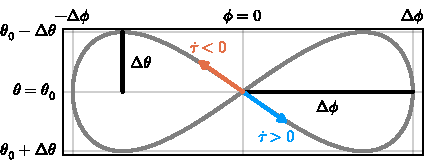
\includegraphics[width=0.6\textwidth]{figs/eight_plot}
  %\caption{The lemniscate that forms the base of the cone of constraints for the kite motion is parameterized by $\tau$ and its shape is controlled by design parameters $\theta_0$, $\Delta\theta$ and $\Delta \phi$. If $\tau$ increases (blue), the kite ascends in the middle and descends on the sides, while it is the opposite for a decreasing $\tau$ (orange). $\tau$ is increasing for a kite that ascends in the middle and descends on the sides (blue) while it is decreasing for the opposite (orange). The $y$-axis is flipped to reflect the orientation of the kite's trajectory.}
  \caption{The lemniscate, which forms the base of the kite's cone of constraints, is parameterized by $\tau$ and its shape is controlled by the design parameters $\theta_0$, $\Delta\theta$, and $\Delta\phi$. Trajectories with increasing $\tau$ (blue) result in a flight path that ascends in the middle and descends at the sides, while decreasing $\tau$ (orange) produces the inverse motion. The $y$-axis is inverted to align with the orientation of the kite's trajectory.}
  \label{fig:eight_plot}
\end{figure}

where \( \tau \in  \mathbb{S}^1 \), \( \theta_0 \) is the mean polar angle, and \( \Delta \theta \) and \( \Delta \phi \) are the amplitudes of the polar and azimuthal oscillations, respectively.

\begin{figure}
  \centering
  \includestandalone[width=0.6\textwidth]{figs/configuration}
  \caption{Configuration of the system. The vector $\mathbf{OA}$ represents the arm, connected at point $A$ (tip of the arm) to the kite $K$ by the lines $\mathbf{AK}$.}
  \label{fig:config}
\end{figure}

\begin{figure} 
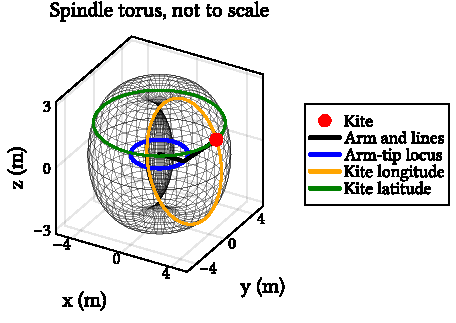
\includegraphics[width=0.6\textwidth]{figs/spindle_torus}

\alter{remove title, labels, tick labels, rescale properly ?}
\end{figure}

The fixed length of the lines imposes a geometric constraint. Defining \( \vb \ell = \AK \), we get
\begin{equation} \label{eq:loop}
    \boldsymbol{\ell} = \vb r - \vb a  \mathbf{\ell}  \text{\alter{ vb ell and ell result in the same glyph. use $\underline{\ell} ?$}}
\end{equation}
which, using \(\norm{\vb\ell}=\ell\), yields
\begin{equation}
    \ell^2 - r^2 + 2 r \vu r \vdot \vb a - a^2 = 0.
\end{equation}
Introducing the projection of the arm onto the radial direction, 
$$
p(\alpha, \tau) = \vu r \vdot \vb a = = a \sin\theta(\tau) \cos(\phi(\tau) - \alpha), $$
the constraint becomes
\begin{equation}
    r^2 - 2 p(\alpha, \tau) r + a^2 - \ell^2 = 0.
\end{equation}
Choosing the positive root corresponding to the kite above ground gives
\begin{equation}
    r(\alpha, \tau) = p(\alpha, \tau) + \sqrt{p(\alpha, \tau)^2 + \ell^2 - a^2}.
\end{equation}
Consequently, the position of the kite is entirely given by
\begin{equation}
    \vb r(\alpha, \tau) = r(\alpha, \tau) \vu r(\tau) 
\end{equation}
We therefore choose \(\vq=(\alpha,\tau)\) as generalized coordinates, which fully describe the configuration of the system.
The corresponding generalized velocities are
\(\dq=(\dot\alpha,\dot\tau)\). The velocity of the arm tip is
\begin{equation}
    \dot{\vb a} = \pdv{\vb a}{\vq} \dq
    = \begin{pmatrix} -a \sin \alpha & 0 \\ a \cos \alpha & 0 \\ 0 & 0 \end{pmatrix} \begin{pmatrix} \dot{\alpha} \\ \dot{\tau}  \end{pmatrix}
    = a \begin{pmatrix} -\sin \alpha \\ \cos \alpha \\ 0 \end{pmatrix} \dot \alpha,
\end{equation}
while the velocity of the kite is:
\begin{equation}
    \dot{\vb r} = \pdv{\vb r}{\vq} \dq
\end{equation}
The latter expression is kept in implicit form to streamline the flow of the discussion. Derivatives can be obtained for numerical implementation purposes via \ac{ad}.

\alter{clarify}

\alter{add definition of power and work. Copied from \textbf{section3-optimization.tex}
The average power is given by
\begin{equation}
    \bar P = W_f/t_f
\end{equation} where \(W_f\) is the total work done during one limit cycle and \(t_f\) is its period. We augment the state of our dynamical system with \(W\) that verifies:
\begin{equation}
\begin{cases}
    W(0) = 0 \\
    \dot W(t) = \dot W(t) = - \dot \alpha \, T(\dot \alpha) = b \, \dot \alpha^2 \quad (\geq 0),
\end{cases}
\end{equation}
}

% \begin{equation}
%     \dot{\vb r} = \pdv{\vb r}{\alpha} \dot{\alpha} + \pdv{\vb r}{\tau} \dot{\tau}.
% \end{equation}
% The partial derivatives of the radial distance \( r(\alpha, \tau) \) are given by:
% \begin{equation}
%     \pdv{r}{\alpha} = \pdv{p}{\alpha} \frac{r}{\sqrt{p^2 + \ell^2 - a^2}}, \quad \pdv{r}{\tau} = \pdv{p}{\tau} \frac{r}{\sqrt{p^2 + \ell^2 - a^2}}
% \end{equation}
% where the partial derivatives of \( p(\alpha, \tau) \) are:
% \begin{align}
%     \pdv{p}{\alpha} &= a \sin\theta(\tau) \sin(\phi(\tau) - \alpha) \\
%     \pdv{p}{\tau} &= a \theta'(\tau) \cos\theta(\tau) \cos(\phi(\tau) - \alpha) - a \phi'(\tau) \sin\theta(\tau) \sin(\phi(\tau) - \alpha)
% \end{align}
% with the derivatives of the spherical coordinates relative to the curve parameter \( \tau \) defined as:
% \begin{equation}
%     \theta'(\tau) = 2 \Delta\theta \cos(2\tau), \quad \phi'(\tau) = \Delta\phi \cos(\tau).
% \end{equation}
% The derivative of the unit radial vector \( \vu r(\tau) \) is:
% \begin{equation}
%     \dv{\vu r}{\tau} = \begin{pmatrix} 
%         \theta'(\tau)\cos\theta(\tau)\cos\phi(\tau) - \phi'(\tau)\sin\theta(\tau)\sin\phi(\tau) \\ 
%         \theta'(\tau)\cos\theta(\tau)\sin\phi(\tau) + \phi'(\tau)\sin\theta(\tau)\cos\phi(\tau) \\ 
%         -\theta'(\tau)\sin\theta(\tau) 
%     \end{pmatrix}.
% \end{equation}

\subsection{Force model}
%kite:
% - inertia
% - gravity
% - aero
% - line tension
% - fictitious cone force
%arm:
% - inertia
% - resistive torque
% - line torque

We model the wind velocity profile \( \vb w \) using a standard power-law wind shear model \addcite{1/7 power law}. Since the unit vector \( \vu x \) points downwind, the wind field is given by:
\begin{equation}
    \vb w(z) = w_{\text{ref}} \qty(\frac{z}{z_{\text{ref}}})^{1/7} \vu x
\end{equation}
where \( w_{\text{ref}} \) is the reference wind speed at altitude \( z_{\text{ref}} \). The altitude of the kite, $z$, is given by
\begin{equation}
    z = \vb r \vdot \vu z = r(\alpha, \tau) \cos\theta(\tau).
\end{equation}
The apparent wind velocity experienced by the kite is thus
\begin{equation}
    \vb w_a = \vb w(z) - \dot{\vb r}.
\end{equation}


The kite is subject to gravity, aerodynamic force, line tension, and the residual force constraining its prescribed conical motion. Gravity is modeled as
    \begin{equation} \label{eq:f_grav}
        \vb F_g = -\qty(m + \frac{m_\ell}{2}) g \vu z
    \end{equation}
where \(m_\ell = n \pi \ell \rho_\ell d_\ell^2 / 4\) is the total mass of the lines, half of which is assumed to be lifted by the kite.

The aerodynamic resultant is computed from the apparent wind using the same model detailed in Section~\ref{sec:model10D-dyn-aero}, namely:
    \begin{equation} \label{eq:f_aero}
        \vb F_a = L \vu k_t + D \vu k_b + \tilde D_\ell \vu k_b,
    \end{equation}
where the lift \(L\) and drag \(D\) are proportional to \(\norm{\vb w_a}^2\), and the line drag \(\tilde D_\ell\) is given by the integral approximation provided in Appendix~\ref{refappendix}.

The arm rotates about the axis \(\Delta = (O, \vu z)\) with moment of inertia \(I\).
It is subject to the torque exerted by the lines at $A$, and to the resistive torque of the generator, modeled as
\begin{equation}
    T(\dot\alpha)=-b\dot\alpha.
\end{equation}
The force exerted by the lines on the arm is \(-\vb F_\ell\), whose moment about \(\Delta\) is
\begin{equation} \label{eq:moment_fell}
        M_\Delta(-\vb F_\ell) = a F_\ell \lhat \vdot (\vu z \times \ahat).
\end{equation}
Newton's second law for the arm yields
\begin{equation} \label{eq:newton_arm}
    I \ddot\alpha = a F_\ell \lhat \vdot (\vu z \times \ahat) - T(\dot \alpha),
\end{equation}
    \alter{Error +T or \(T=b\dot{\alpha} \, with\, b>0\)}
from which the line tension is expressed as
    \begin{equation} \label{eq:f_lines}
        F_\ell = \frac{-I \ddot\alpha - T(\dot \alpha)}{a \lhat \vdot (\vu z \times \ahat)},
        \qquad
        \vb F_\ell = -F_\ell \lhat.
    \end{equation}

\subsection{Equations of motion}
The prescribed trajectory of the kite is enforced through a frictionless geometric constraint. The corresponding  eight-shaped coneical shape is
    \begin{equation}
        \mathcal{C} = \{\, R \rhat(\tau) \mid R>0,\ \tau\in[0,2\pi) \,\}.
    \end{equation}
Its tangent space is spanned by \(\partial\OK/\partial R = \rhat\) and \(\partial\OK/\partial\tau = R \rhat'\).
According to d'Alembert's principle, the constraint force, \(\vb F_c\), performs no virtual work along admissible displacements, so that:
    \begin{equation} \label{eq:cone_constraint}
        \vb F_c \vdot \rhat = 0,\qquad
        \vb F_c \vdot \rhat' = 0.
    \end{equation}
Newton's second law for the kite reads
    \begin{equation} \label{eq:newton_kite}
        m \ddot{\vb r} = \vb F_a + \vb F_g + \vb F_\ell + \vb F_c.
    \end{equation}
Combining this equation with the arm's dynamics and eliminating the constraint force using \eqref{eq:cone_constraint} yields a \(2\times2\) linear system for the generalized accelerations:
    \begin{equation} \label{eq:eom_implicit}
        M(\vq) \ddq = \vb h(\vq, \dq),
    \end{equation}
    whose explicit solution is derived in Section~\ref{sec:explicit-ddq} \alter{keep that annex?}.

\alter{Lonely sentence} We write the state of the dynamical system \(vb x = (\vq, \dq) = (\alpha, \tau, \dot \alpha, \dot \tau\) and define the evolution function \(f\) as
\begin{equation}
    f(\vb x) = f(\vq, \dq) = (\dq, \ddq),
\end{equation}
where \(\ddq\) is solution to \ref{eq:eom_implicit}.
The system is symmetric through the map
\begin{equation}
\label{eq:symmetry}
    \sigma: (\alpha, \tau, \dot \alpha, \dot \tau) \mapsto (-\alpha, \tau + \pi, -\dot \alpha, \dot \tau)
\end{equation}

The mechanical power extracted by the generator is
\begin{equation}
    \dot W(t)
    = -\dot\alpha\,T(\dot\alpha)
    = b\dot\alpha^2\geq0,
\end{equation}
where \(W(0)=0\). The average power of a solution spanning \([0, t_f]\) is
\begin{equation}
    \bar P=\frac{W_f}{t_f},
\end{equation}
where \(W_f=W(t_f)\) is the total extracted work.










% We apply Newton's second law of motion to the kite :
% \begin{equation}
%     \sum \vb F_i = m \dot{\vb r}
% \end{equation}

% All force formulas derived in \ref{sec:model10D-dynamics} still apply here, except for \ref{eq:newton_arm} because \( \theta \) and \( \phi \) are not defined anymore.
% % Why ?
% % The relationship between the line tension at \( A \) — \( -\vb F_\ell = - F_\ell \lhat \), and the moment it applies on the arm around axis \( \Delta = (O, \vu z) \) passing through \( O \) with direction \( \vu z \) — \( M_\Delta(-\vb F_\ell) \), 
% Instead of computing these angles from the \( q \), we derive a new formula:
% \begin{equation}
%     M_\Delta(\vb F_\ell) = a F_\ell \lhat \vdot (\vu z \times \ahat)
% \end{equation}

% \begin{proof}
% The lines apply of force \( -\vb F_\ell \) on the arm \( \OA \) at point \( A \), which rotates around \( \Delta \).
% The corresponding moment is
% \begin{equation}\begin{split}
%     M_\Delta(-\vb F_\ell) &= \vb M_O(-\vb F_\ell) \vdot \vu z = [\OA, -\vb F_\ell, \vu z] = [a \ahat, F_\ell \lhat, \vu z] = a F_\ell [\lhat, \vu z, \ahat] \\
%     &= a F_\ell \lhat \vdot (\vu z \times \ahat),
% \end{split}
% \end{equation}
% where \( [\vb a, \vb b, \vb c] = (\vb a \times \vb b) \vdot \vb c \) denotes the triple product, which is invariant under circular shift, and \( \vu z \times \ahat \) is simply \( (-\sin(\alpha), \cos(\alpha), 0) \).


% \alter{<remove label="circular shift proof">}
% We write \( \lhat \) in the base attached to the arm \( (\ahat, \vu z \times \ahat, \vu z) \):
% \begin{equation}
%     \lhat = (\lhat \vdot \ahat) \ahat + (\lhat \vdot (\vu z \times \ahat)) (\vu z \times \ahat) + (\lhat \vdot \vu z) \vu z
% \end{equation}
% to easily develop the triple product into
% \begin{equation}
%     M_\Delta(\vb F_\ell) = (a \ahat \times F_\ell \lhat) \vdot \vu z = a F_\ell \lhat \vdot (\vu z \times \ahat).
% \end{equation}
% \alter{</remove>}
% \end{proof}

% \subsection{Newton's second law}
% The arm has inertia \( I \) and the electrical generator applies torque \( T : \omega \mapsto -b \omega \) where b is analogous to a rotational viscous damping coefficient, with dimension of torque per angular velocity.
% Applying Newton's second law to the arm gives
% \begin{equation}
%     I \ddot \alpha = M_\Delta(\vb F_\ell) + T(\dot \alpha) = \alpha F_\ell \lhat \vdot (\vu z \times \ahat) - b \dot \alpha,
% \end{equation}
% from which we obtain \( \vb F_\ell \), pointing from the \( K \) to \( A \), thus in the direction of \( -\lhat \):
% \begin{equation} \label{eq:f_lines}
%     \vb F_\ell = \frac{-I \ddot \alpha - b \dot \alpha}{a \lhat \vdot (\vu z \times \ahat)} \lhat
% \end{equation}

% \alter{put this at the right place}
% The wind profile is parameterized by \( z_0 \), a reference altitude, and \( w_0 \), its speed at this altitude.
% Using the 1/7th power rule \alter{\url{https://journals.ametsoc.org/view/journals/apme/17/3/1520-0450_1978_017_0390_otuopl_2_0_co_2.pdf}}, we obtain
% \begin{equation}
%     \vu w(z) = w_0 (\frac{z}{z_0})^\frac{1}{7} \vu x.
% \end{equation}


% The forces applied to the kite are:
% \begin{itemize}
%     \item gravity \( \vb F_g = -(m + m_\ell/2) g \vu z \)
%     \item aerodynamic resultant \( \vb F_a = L \vu k_t + (D + \tilde D_\ell) \vu k_b \), the detailed computation is found in \ref{sec:model10D-dyn-aero}
%     \item line tension \( \vb F_\ell \) computed in \ref{eq:f_lines}
%     \item the fictitious cone force \( \vb F_c \) that still needs to be determined.
% \end{itemize}

% We apply Newton's second law to the kite and isolate \( \vb F_c \)
% \begin{equation} \label{eq:f_cone_newton}
%     \vb F_c(\vq, \dq, \ddq) = m \ddot \OK(\vq, \dq, \ddq) - \vb F_g - \vb F_a(\vq, \dq) - \vb F_\ell(\vq, \dq, \ddq).
% \end{equation}
% For the kite to stay on the eight-shaped cone, we choose \( \vb F_c \) to be the solution of
% \begin{equation}\begin{cases} \label{eq:f_cone_constraint}
%     \vb F_c \vdot \pdv{\OK}{R} = 0 \\
%     \vb F_c \vdot \pdv{\OK}{\tau} = 0
% \end{cases}\end{equation}
% \alter{use \( \tilde \OK(R, \tau) \) instead of \( \OK(\alpha, \tau) \) ? Should I even keep \( \tilde \OK \) ? It's more mechanics than maths}
% so that the kite glides without friction on the cone.
% Given some generalized coordinates \( \vq \) and velocities \( \dq \), this system of \( 2 \) equations can be solved for the accelerations \( \ddq \in \R^2 \), therefore defining a second order \ac{ode} on \( \vq \).

% Let's compare this result to that of \ref{sec:model10D}.
% We had a \ac{dae} of dimension \( 5 \) with \( 2 \) \ac{dof} and \( 3 \) constraints, while by computing essentially the same quantities but only using generalized coordinates \( \vq = (\alpha, \tau) \), we have an easier problem to solve with fewer calculations.
% We go a step further by solving this system without a symbolic solver, thus writing \( \ddq \) explicitly in terms of \( \vq \) and \( \dq \); see \ref{sec:explicit-ddq} for the detailed calculation.
% The result is
% \begin{equation}
%     2
% \end{equation}
\section{Estimation of power take-off} \label{sec:1D-PTO}
A simple 1D dynamic model is derived in order to estimate the \ac{pto} by the KEEP device, that is the mechanical power extracted from the rotation of the arm by the generator, modelled as a viscous torque \(-b\dot\alpha\) (average of \(b\dot\alpha^2\)). Significant assumptions are made. An \(\omega\)-pulsation harmonic couple around \(\vu z\), caused by the tether attached to the end of the arm, is modelled by \(C_M\,\cos(\omega\,t)\), where \(C_M=F_s\,a \sin \theta_0\) and \(F_s\) is a constant tension in the line. Thus, the variation of the aerodynamics forces along the kite’s figure-of-eight trajectory is averaged and projected onto the horizontal plane (\(z=0\)). The Newton's second law for the arm \ref{eq:newton_arm} yields
\begin{equation} \label{eq:newton_arm_PTO}
    I \ddot\alpha = C_M\,\cos(\omega\,t) -b \dot\alpha.
\end{equation}
The following non dimensional parameters \(\overline{b}=b/(I\,\omega)\), \(\overline{C_M}=C_M/(I\,\omega^2)\) and \(\tau=\omega\,t\) are defined. The derivative of \(\alpha\) with respect to \(\tau\) is denoted by \(\alpha'\), such that \(\alpha'=\dot{\alpha}/\omega\). The Newton's second law for the arm \ref{eq:newton_arm_PTO} simplifies as follows
\begin{equation} \label{eq:newton_arm_PTO_adim}
    \alpha''+\overline{b}\, \alpha' = \overline{C_M}\,\cos(\tau).
\end{equation}
The steady-state harmonic solution of \ref{eq:newton_arm_PTO_adim} is
\begin{equation} \label{eq:sol_alpha_PTO}
    \alpha = -\frac{\overline{C_M}}{B}\,\cos(\tau+\delta),
\end{equation}
where \(B=(1+\overline{b}^2)^{1/2}\) and \(\delta=\arctan \overline{b}\). This last relationship shows that the phase difference between the angular position of the arm and that of the kite is closely linked to the rotor resistance $b$. The mechanical power produced by the device is expressed as
\begin{equation} \label{eq:inst_power_PTO}
    \dot{W} = b \, \dot \alpha^2=I\,\omega^3\,\overline{b}\,\alpha'^2.
\end{equation}
Consequently, the average power produced over a steady-state operating cycle of the KEEP system is given by
\begin{equation} \label{eq:power_PTO}
    W_a =  \frac{1}{2\pi}\,\int \limits_{\tau=0}^{\tau=2\pi} \dot{W} \dd{\tau}=\frac{\overline{b}}{2\,\left(1+\overline{b}^2\right)}\, \frac{{C_M}^2}{I\,\omega}.
\end{equation}
A maximum tension condition is imposed on the cable whilst seeking to preserve the structural integrity of the kite (maximum stress, local buckling of the inflatable tubes, etc.) \cite{Desenclos2023MCM}. Denoting \(F_s\) the maximum tension, it is generally expressed as \(F_s=T_s\, S\), where \(T_s\) is a maximum wing loading independent of the kite’s surface area \(S\). Thus, the amplitude of the harmonic couple \(C_M\) can be expressed as follows:
\begin{equation} \label{eq:C_M_PTO}
    C_M=T_s\, S\,a \sin(\theta_0).
\end{equation}
Furthermore, the pulsation \(\omega\) introduced in the simple formulation \ref{eq:newton_arm_PTO} can be determined using a zero-mass model of the  kite \cite{Leloup2014OE}. We consider line length \(\ell\) that are much greater than the arm length \(a\), so that \(r=\ell\) is a reasonable assumption. Futhermore, assuming a constant kite speed \(V_k=\lVert \dot{\boldsymbol{r}} \rVert\) along its figure-of-eight trajectory, equal to the value at the center \((x,y,z)=(\ell\,\sin(\theta_0),0,\ell\,\cos(\theta_0))\), it can be shown that 
\begin{equation} \label{eq:Vk_PTO}
    V_k=w_\ell\,\left(\frac{\ell\,\cos(\theta_0)}{z_r}\right)^{1/7}\,\sqrt{\left(1+G^2\right)\,{\sin(\theta_0)}^2-1},
\end{equation}
where \(G=C_L/C_D\) is the glide ratio of the kite. According to \ref{eq:sphere_Model_Deriv} and \ref{eq:traject_Model_Deriv}, the total length of the figure-of-eight trajectory \(L_{81}\) on the unit sphere (\(\ell=1\)) is given by
\begin{equation} \label{eq:L81_PTO}
    L_{81}=\int \limits_{\tau=0}^{\tau=2\pi} \sqrt{\left[2 \, \Delta\theta\, \cos(2\,\tau)\right]^2+{\sin(\theta_0 + \Delta\theta \sin(2\tau))}^2\,\left[\Delta\phi\, \cos(\tau)\right]^2} \dd{\tau},
\end{equation}
hence the following expression of the pulsation
\begin{equation} \label{eq:Omega_PTO}
    \omega=\frac{2\,\pi\,V_k}{\ell\,L_{81}}.
\end{equation}
As detailed in appendix \ref{app8}, one has the following estimate:
\begin{equation} \label{eq:L81_PTO_approx}
L_{81}=4\Delta\phi\sin\theta_0+\frac{8\,\Delta\theta^2}{\Delta\phi\sin\theta_0}\Bigl[\ln\frac{2\Delta\phi\sin\theta_0}{\Delta\theta}-\frac56-\frac2{15}\Delta\phi^2\sin^2\theta_0\Bigr]+o(\Delta\theta^2).
\end{equation}
Assuming that the values of the aerodynamics parameters \(G\), \(w_r\) and \(z_r\), of the geometry parameters \(a\), \(\ell\), \(\theta_0\), \(\Delta \theta\) and \(\Delta \phi\), as well as those of the kite properties \(S\) and \(T_s\), have been selected, the independent parameters \(b\) and \(I\) can be optimized.
At fixed inertia \(I\), the last term of the relationship (\ref{eq:power_PTO}) reaches its maximum value for \(\overline{b}=1\), that is
\begin{equation} \label{pto_optimality_constraint}
    b=I\,\omega,
\end{equation}
which gives the average power \(W_a = C_M^2/(4I\omega)\).
For operating reasons, the magnitude of the angle \(\alpha\) is limited to \(\pi/2\). By~\eqref{eq:sol_alpha_PTO}, the amplitude is \(\overline{C_M}/B = C_M/(\omega\sqrt{I^2\omega^2+b^2})\), hence the condition
\begin{equation} \label{eq:opti_I_PTO}
    \omega^2\qty(I^2\omega^2 + b^2) \geqslant \qty(\frac{2\,C_M}{\pi})^2,
\end{equation}
which depends on both parameters.
With \(Z = I^2\omega^2+b^2\), the power~\eqref{eq:power_PTO} reads \(W_a = b\,C_M^2/(2Z)\).
At fixed \(Z\), it increases with \(b\), that is as \(I\) decreases, and at fixed \(b\) it decreases with \(Z\): in this model, the inertia of the arm only costs power, and the supremum \(\pi C_M\omega/4\) is approached as \(I\to0\), with~\eqref{eq:opti_I_PTO} active.
The inertia is bounded below by the structure of the arm, \(I\geq I_{\min}\), with \(I_{\min} = \SI{62}{\kilogram\meter\squared}\) the lower bound of Table~\ref{tab:opt_descr} (a tube that withstands the maximum tension of the lines).
% I_min: src/optimization.jl, I_BOUNDS (the same bound as the optimization of Section 4)
As long as \(I_{\min} < \sqrt2\,C_M/(\pi\omega^2)\), which holds here, the condition~\eqref{eq:opti_I_PTO} is active at the optimum, and the parameters \(b\) and \(I\) are optimal when
\begin{equation} \label{eq:opti_b_I_PTO}
    I = I_{\min}, \qquad b = \frac{2\,C_M}{\pi\,\omega}\sqrt{1-\varepsilon^2}, \qquad \varepsilon = \frac{\pi\,\omega^2 I_{\min}}{2\,C_M},
\end{equation}
where \(C_M\) and \(\omega\) are given by \ref{eq:C_M_PTO} and \ref{eq:Omega_PTO} respectively, which leads to the following average power:
\begin{equation} \label{eq:opti_power_PTO_final}
    W_a =\frac{\pi\,C_M\,\omega}{4}\sqrt{1-\varepsilon^2}.
\end{equation}
The design \(b = I\omega\) with the smallest admissible \(I\), \(I = \sqrt2\,C_M/(\pi\omega^2) = \SI{\PtoISeq}{\kilogram\meter\squared}\), satisfies the constraint but gives only \(\pi C_M\omega/(4\sqrt2)\): the condition~\eqref{pto_optimality_constraint} is optimal at fixed \(I\), not jointly, and the optimum~\eqref{eq:opti_b_I_PTO} gives \(\PtoGainSeq\,\%\) more power.
Thus, the power take-off per unit area of kite \(pto\) by the KEEP device can be estimated as follows:
\begin{equation} \label{eq:pto_PTO}
    pto=\frac{W_a}{S}=\left(\frac{\pi^2\,\sin(\theta_0)\,\sqrt{\left(1+G^2\right)\,{\sin(\theta_0)}^2-1}}{2\,L_{81}}\right)\,\left(\frac{T_s\,a\,w_r}{\ell}\right)\,\left(\frac{\ell\,\cos(\theta_0)}{z_r}\right)^{1/7}\sqrt{1-\varepsilon^2}.
\end{equation}
The maximum power take-off varies almost linearly with the glide ratio of the kite. The linear dependence of \(pto\) on wind speed \(w_r\) is due to the structural constraint \(T_s\). Without this constraint, the dependence of \(pto\) on wind speed \(w_r\) is normally of the third order, since the aerodynamic pressures – and therefore the wing loading  – are of the second order. The \(pto\) appears to increase linearly as the arm length \(a\) increases. The shorter the length of the line \(\ell\), the higher \(pto\) is, even if the wind speed at the height of the kite decreases. However, the inertia of the kite is not taken into account in this estimate of the power take-off. Taking it into account could alter the value of the pulsation \(\omega\) and, consequently, lead to an optimal value for the length of the line. Taking the nominal parameters of Table~\ref{tab:params} with \(T_s = \SI{\PtoTs}{\newton\per\square\meter}\), \(\varepsilon = \PtoEps\), and the KEEP device achieves a maximum power take-off of about \(\SI{\PtoPower}{\kilo\watt\per\square\meter}\) (\SI{\PtoPowerZero}{\kilo\watt\per\square\meter} as \(I_{\min}\to0\)), regardless of whether expression \ref{eq:L81_PTO} or \ref{eq:L81_PTO_approx} is used for $L_{81}$. The values required for the moment of inertia \(I\) of the arm and the resistance \(b\) of the rotor are \(\SI{\PtoI}{\kilogram\meter\squared}\) and approximately \(\SI{\PtoB}{\newton\meter\second\per\degree}\) respectively.


\begin{table}[thpb]
\centering
\caption{Parameter Description and Values}
\label{tab:params}
\begin{tabular}{l p{3.2cm} r l}
    \toprule
    {Symbol} & {Description} & {Value} & {Unit} \\
    \midrule
    $a$ & Arm length & $2$ & \si{\meter} \\ 
    $b$ & Arm braking coefficient & $50.4063585$ & \si{\newton\meter\second\per\degree} \\ 
    $C_D$ & Kite drag coefficient & $C_L / 7$ &  \\ 
    $C_{D,\ell}$ & Line drag coefficient & $0$ &  \\ 
    $C_L$ & Kite lift coefficient & $0.6$ &  \\ 
    $d_\ell$ & Line diameter & $0.003$ & \si{\meter} \\ 
    $g$ & Gravity & $9.81$ & \si{\meter\per\square\second} \\ 
    $I$ & Arm inertia & $1300$ & \si{\kg\square\meter} \\ 
    $\ell$ & Line length & $31$ & \si{\meter} \\ 
    $m$ & Kite mass & $6$ & \si{\kg} \\ 
    $S$ & Kite surface & $10$ & \si{\square\meter} \\ 
    $w_0$ & Wind reference speed & $9$ & \si{\meter\per\second} \\ 
    $z_0$ & Wind reference altitude & $10$ & \si{\meter} \\ 
    $\Delta\theta$ & Lemniscate polar half-height & $6$ & \si{\degree} \\ 
    $\Delta\phi$ & Lemniscate azimuthal half-width & $50$ & \si{\degree} \\ 
    $\theta_0$ & Lemniscate mean polar angle & $65$ & \si{\degree} \\ 
    $\rho_a$ & Air density & $1.225$ & \si{\kg\per\cubic\meter} \\ 
    $\rho_\ell$ & Line density & $707$ & \si{\kg\per\cubic\meter} \\ 
    \bottomrule
\end{tabular}
\end{table}


\section{Analysis of the dynamics -- equilibria and periodic orbits}

\begin{enumerate}
\item \textbf{Choosing parameters} Set parameters to physically sensible values. Choose $b$ according to optimality criterion \ref{pto_optimality_constraint}.

[Table of parameter values]

\item \textbf{Equilibria}

but first, let's study the equilibria

Define the \ac{bvp} that we are solving, explain why tauf = tau0 + 2pi

First return map converges, look at floquet exponents ?

\item \textbf{General behavior}

    hints at existence of two stable limit cycles

\item \textbf{Limit cycles}

\item \textbf{Algorithm for obtaining a limit cycle}

start form equilibrium, speed in correct direction, integrate until first return map converged.

\end{enumerate}

% TODO relevant? any implications?
All state and parameter values are normalized with unit length \(L\) the physical arm length, unit mass \(M\) the mass of the kite, and unit time \(T\) the wind speed at reference altitude over arm length ratio; therefore, \(a = m = v_{\mathrm{ref}} = 1\).

Let the state be \(vb x = (\vb q, \dq) = (\alpha, \tau, \dot \alpha, \dot \tau\). We are first interested in the steady states of the dynamical system, \emph{i.e.} static solutions with both zero velocity and acceleration. Therefore we are looking for solutions \(\vb q_0\) to

\begin{equation}
    \ddq(\vb q_0, \dq = 0) = 0 \in \R^2.
\end{equation}

In Figure~\ref{fig:equilibria-phase-space} we identify those solutions at the intersections of accelerations in \(\alpha\) and in \(\tau\): 4 null-clines for \(\ddot \tau\) that traverse the plot area horizontally and 2 for \(\ddot \alpha\) that traverse it vertically, therefore this system has \(4 \times 2 = 8\) steady states. We represent the configuration of the system at the steady states in Figure~\ref{fig:equilibria-eight-circle}.


\begin{figure}[thpb]
    \centering
    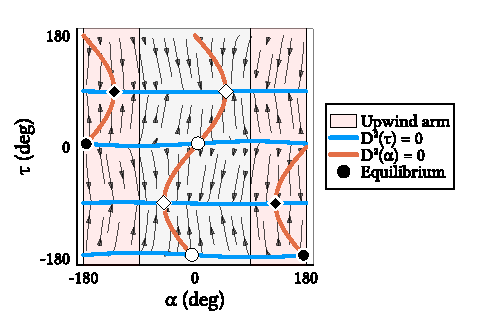
\includegraphics{figs/equilibria_phase_space}
    \caption{Zero velocity curves and equilibria of the dynamics.
    The black arrows represent the direction of the vector field $\ddq(\vq, \dq = 0)$, the green lines are the nullclines of $\ddot \alpha(\alpha, \tau)$, \emph{i.e.} the points $(\alpha, \tau)$ such that $\ddot \alpha(\alpha, \tau) = 0$, and the purple lines are the ones of $\ddot \tau(\alpha, \tau)$.
    At their intersections lie the equilibria of the system (all unstable), with color codes ranging from yellow to blue according to the highest real part of their eigenvalues.
    % TODO change graphical references in captions, also, says that max(Re(lambda i)) is approx 3 for circle and 12 for diamonds, for both colors
    The background is green when the arm points downwind and red when it points upwind.}
    \label{fig:equilibria-phase-space}
\end{figure}

\begin{figure}[thpb]
    \centering
    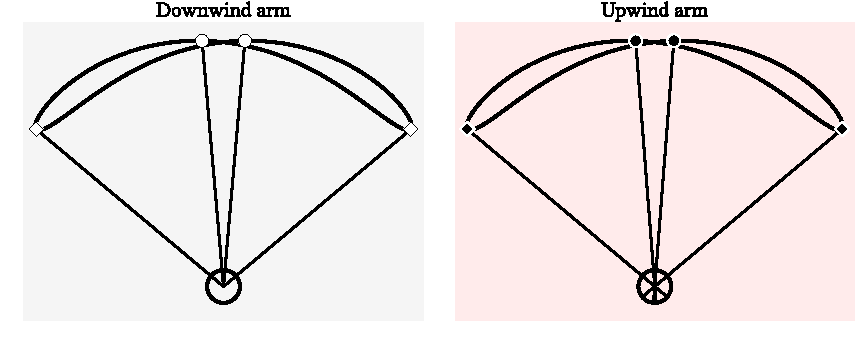
\includegraphics{figs/equilibria_eight_circle}
    % TODO For sale
    \caption{Configuration of the same equilibria in \emph{almost physical} top view of the system (the position of the kite is not adjusted according to the arm angle). We verified numerically that for all equilibria, the arm and the lines belong to the same vertical plane, \emph{i.e.} their projections in the $XY$ plane are aligned.}
    We find eight equilibria in total. They are unstable and we verify that for all of them, the lines and the arms are aligned when projected in the $x-y$ plane.
    % TODO move steady states descriptions here: one ss on the side (diamond), one near the center (circle), plus their symmetry through sigma (eq:symmetry), for both downwind and upwind arm.
    \label{fig:equilibria-eight-circle}
\end{figure}

Let us now look at dynamical solutions to this dynamical system. One such trajectory is a solution to

\begin{equation}
    \dot x = f(x)
\end{equation}
% TODO cite OrdinaryDiffEqVerner.jl
For integrating, we use the order-9 Verner method provided by OrdinaryDiffEqVerner.jl with absolute and relative integration tolerance of \(10^{-9}\) unless specified otherwise.

% TODO or adimensionalized?
Let \( x_0^{\pm} = (0, 0, 0, \pm 1)\) in normalized units. Time series for \(x_0^+\) exhibit a periodic orbit behavior.  

\begin{figure}[thpb]
    \centering
    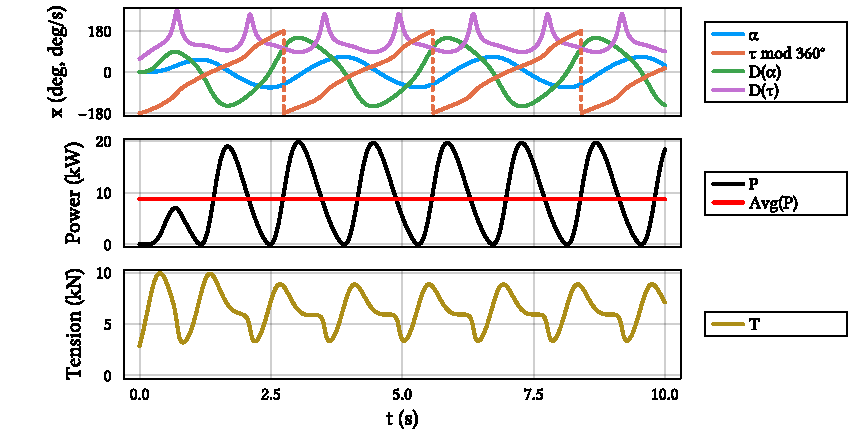
\includegraphics{figs/time_series_4D}
    % TODO give the initial state
    \caption{Time series of the state for a ten second integration. After a few seconds, the same pattern is repeated: this hints that our dynamical system exhibits a limit cycle.}
    \label{fig:timeseries}
\end{figure}



\begin{figure}[thpb]
    \centering
    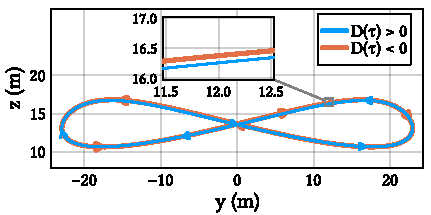
\includegraphics{figs/yz_limit_cycles}
    \caption{Projection of the kite trajectories onto the $YZ$ plane for the two limit cycles with opposite directions of motion (arrows indicate the direction of the kite motion). Zooming in on the trajectories shows that the two paths are distinct}
    \label{fig:yz_limit_cycle}
\end{figure}

Deflation algorithm for that set of parameters did not yield new limit cycles, on top of the two that are obtained with \(x_0^\pm\).


We define a sequence of states $(\vb x_i)_{i \geq 1}$ lying on a surface of section $\Sigma$, such that $\vb x_{i+1}$ is the first intersection between $\{\varphi^t(\vb x_i),\, t > 0\}$ and $\Sigma$, where $\varphi^t$ is the flow of ~\eqref{eq:eom}. Let
\begin{equation}
    \Sigma = \{\vb x \in T\mathbf{T}^2 \mid \tau(\vb x) = 0\}
\end{equation}
and $\Delta t(\vb x)$ be the time needed to achieve the first crossing of $\Sigma$ from state $\vb x$, namely:
\begin{equation}
    \Delta t(\vb x) = \min\{t > 0 \mid \varphi^t(\vb x) \in \Sigma\}.
\end{equation}
We then define the first recurrence map, or Poincaré map, as
\begin{equation}
    P : \vb x \in T\mathbf{T}^2 \mapsto \varphi^{\Delta t(\vb x)}(\vb x) \in \Sigma,
\end{equation}
and finally the desired sequence
\begin{equation}\begin{cases}
    \vb x_0 = P(\vb x^0) \\
    \vb x_{i+1} = P(\vb x_i).
\end{cases}\end{equation}

Since the trajectory starting at $\vb x^0$ approaches an attracting limit cycle, the limit of this sequence is defined and we plot the distance from $\vb x_i$ to $\vb x_\infty = \lim_{i \to \infty} \vb x_i$ in Figure~\ref{fig:convergence}.
The sequence converges exponentially, and in only $8$ iterations (seven revolutions over the lemniscate), we reach the precision limit of our ODE solver, with a distance of less than $10^{-12}$; in fact, we approximately gain $2$ digits of $\vb x_\infty$ after each revolution.
The points $\vb x_i$ are obtained using DifferentialEquations.jl's continuous callback feature, which saves the current state when a user defined function changes its sign, using the high-precision dense output from the ODE solver.

We confirm that there exist only two attracting limit cycles by sampling the state space with $(\alpha, \tau) \in \mathbf{T}^2$ and velocities $-M \leq \dot\alpha, \dot\tau \leq M$, and simulating the trajectory of each sampled point until convergence to a limit cycle with a \SI{1e-9} tolerance.
We choose $M = 10 \si{\radian\per\second}$ as upper bound; it corresponds to high arm and kite speeds which would be quickly damped by the generator and aerodynamic drag anyway.

\begin{figure}[thpb]
    \centering
    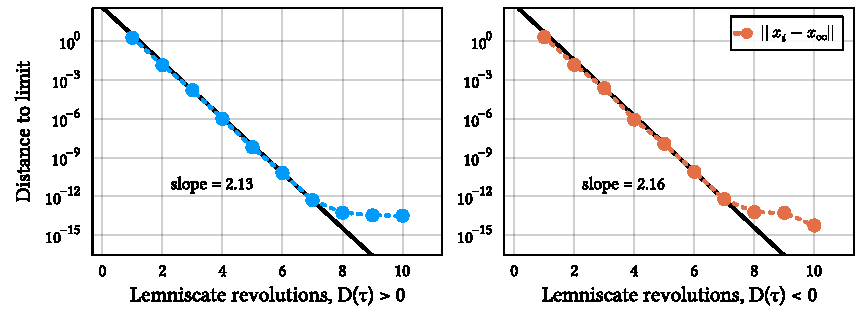
\includegraphics{figs/limit_cycle_convergence}
    \caption{Convergence toward the fixed point on the Poincaré map. The trajectory gets closer to the limit cycle as the number of lemniscate revolutions (a revolution is defined as a sweep over the interval $[0,2\pi]$ for the angle $\tau$) increases.
    The linear trend in log-linear plot indicates exponential convergence; after each revolution, the distance to the limit decreases by a factor of $10^{2.13}$ (\(\dot \tau > 0\)) or \(10^2.16\) (\(\dot \tau < 0\)), until it stalls near the tolerance of the integration scheme, set at \(10^{-13}\). The colored line is for \(\vb q_0 = (0, 0)\), perturbed trajectories are integrated from \(\vb q_0\) sampled in \([0, 2\pi]^2\).}
    \label{fig:limit_cycle_convergence}
\end{figure}

\section{Optimization} \label{sec:optimization}

We designed this model to evaluate the average power output of KEEP.
%\alter{add a label to the dynamical analysis section and reference it}
In the previous section, we computed limit cycles for a given set of environment and design parameters.
%\alter{do we keep 'limit cycle'?}
We now fix the environment, mainly the reference wind speed \(w_0\), and maximize the average power output over one revolution of a periodic orbit by tuning a selection of design parameters.

\subsection{Optimizing for maximum average power} \label{sec:opt-power}

To assess the quality of a set of parameters, we measure the total work done by the generator, \emph{i.e.} the amount of energy extracted from the system.
We obtain this information by augmenting the state with the work \(W\) done since the start of the simulation, whose time derivative is the instantaneous power, namely the product of (the opposite of) the torque and the arm angular velocity:
\begin{equation} \label{eq:work}
    W(0) = 0, \qquad
    \dot W = P = - \dot \alpha \, T(\dot \alpha) = b \, \dot \alpha^2 \geq 0.
\end{equation}
The work is integrated concurrently with \(\vb x = (\alpha, \tau, \dot \alpha, \dot \tau)\), using the same numerical scheme, and we denote the augmented state \(\tilde{\vb x} = (\vb x, W)\).
The average power over a periodic orbit of period \(t_f\) is then
\begin{equation}
    \bar P = W_f / t_f, \qquad W_f = W(t_f).
\end{equation}
Since the trajectory converges to the same periodic orbit (given \(\dot \tau > 0\)), maximizing the average power as \(t \to \infty\) is equivalent to maximizing it over one period of this orbit.

For the solution of the \ac{ivp} to be a periodic orbit, looping constraints must be enforced at \(t_f\), which yields a \ac{bvp}.
Without loss of generality, we fix the phase by imposing \(\tau(0) = 0\), so that \(\tau(t_f) = \pm 2\pi\).
%\alter{this is probably going to be a repeat of the previous section}
The sign determines the direction of travel of the kite: it rises either on the sides of the eight (\(\tau(t_f) = +2\pi\)) or in its center (\(\tau(t_f) = -2\pi\)).
To avoid the lines sliding against each other, we choose the former.

We optimize the line length \(\ell\), the arm inertia \(I\), the braking coefficient \(b\) of the generator and the half-width \(\Delta\varphi\) of the eight, and denote by \(\Theta = (\ell, I, b, \Delta\varphi)\) the vector of design parameters; the half-height \(\Delta\theta = \DthetaFixed^\circ\) of the eight is held fixed.
The optimization problem reads
\begin{equation} \label{eq:opt-problem}
W_f / t_f \underset{\substack{\alpha_0, \dot{\alpha}_0, \dot{\tau}_0 \\ W_f, t_f \\ \Theta}}{\longrightarrow} \max
\end{equation}
subject to constraints
\begin{equation} \label{eq:opt-constraints}
\begin{split}
    &\alpha(t_f, \Theta) = \alpha_0 \\
    &\tau(t_f, \Theta) = 2\pi \\
    &\dot \alpha(t_f, \Theta) = \dot \alpha_0 \\
    &\dot \tau(t_f, \Theta) = \dot \tau_0 \\
    &W(t_f, \Theta) = W_f,
\end{split}
\end{equation}
where the components of \(\tilde{\vb x}(t_f, \Theta)\) are obtained by integrating the \ac{ivp} from \(\tilde{\vb x}_0 = (\alpha_0, 0, \dot \alpha_0, \dot \tau_0, 0)\) with parameters \(\Theta\), and \(W_f\) is a slack variable for the final work.
In the search for parameters that provide more power, the solver thus also determines the corresponding initial condition lying on the periodic orbit.

\paragraph{Initial guess.}
We reuse our work on equilibria and limit cycles to provide the solver with an initial guess that satisfies the constraints.
%\alter{can we get them from Alain's kinematic model in the appendix? ``We start with values obtained from annex X where we use a kinematic model to determine the optimal parameters...''}
Starting from a physically reasonable set of parameters \(\Theta_0\), we compute the corresponding limit cycle (with the correct direction of travel), from which we extract \(\alpha_0, \dot \alpha_0, \dot \tau_0, t_f\) and \(W_f\); this results into a feasible point.

\paragraph{Implementation.}
The problem is modelled with ADNLPModels.jl \cite{migot2021adnlpmodels}, which computes all required derivatives algorithmically with ForwardDiff.jl \cite{RevelsLubinPapamarkou2016}.
It is solved by the interior point method implemented in Ipopt \cite{WachterBiegler2006} (tolerance \(\IpoptTol\)), called through NLPModelsIpopt.jl, with linear solver MUMPS \cite{amestoy2001mumps}.
The \ac{ivp} appearing in the nonlinear constraints is solved at tolerance \(\IvpTol\) with Vern9, Verner's Runge--Kutta 9(8) method from DifferentialEquations.jl \cite{rackauckas2017differentialequations}.
% TODO cite Verner's paper (reference to be checked before adding)
%\alter{Ipopt requires a bounding box; we give it as large as possible to avoid saturating a bound.}
The parameters and their bounds are described in Table~\ref{tab:opt_descr}, while the result of the optimization is presented in Table~\ref{tab:opt_results}.
%\alter{ECC run: 11 iterations, \SI{0.5}{\second} on an M2 MacBook Air, but at tolerance \(10^{-6}\); update iteration count and timing for \(10^{-8}\)}
Ipopt solves the problem in \IpoptIter{} iterations.
We show the limit cycles before and after optimization in Figure~\ref{fig:time_series}: the period goes from \SI{\PeriodInit}{\second} to \SI{\PeriodOpt}{\second}, and the average power from \SI{\PowerInit}{\kilo\watt} to \SI{\PowerOpt}{\kilo\watt} (\(+\PowerGain\%\)).

\begin{table}[thpb]
\centering
\caption{Description of the optimized parameters ($\Delta\theta = \SI{6.0}{\degree}$ fixed).}
\begin{tabular}{l S S}
    \toprule
    {Symbol (Unit)} & {Lower bound} & {Upper bound} \\
    \midrule
    $\ell$ (\si{\meter}) & 15.0 & 200.0 \\ 
    $I$ (\si{\kilogram\meter\squared}) & 62.0 & 1000000.0 \\ 
    $b$ (\si{\newton\meter\second\per\degree}) & 0.0175 & 17453.3 \\ 
    $\Delta\varphi$ (\si{\degree}) & 10.0 & 90.0 \\ 
    \bottomrule
\end{tabular}
\label{tab:opt_descr}
\end{table}


\begin{table}[thpb]
\centering
\caption{Optimization results}
\begin{tabular}{l S S}
    \toprule
    {Symbol (Unit)} & {Initial Guess} & {Solution} \\
    \midrule
    $\ell$ (\si{\meter}) & 31.0 & 47.4 \\
    $I$ (\si{\kilogram\meter\squared}) & 1300.0 & 3541.3 \\
    $b$ (\si{\newton\meter\second\per\radian}) & 4000.0 & 3862.6 \\
    \midrule
    Average power (\si{\kilo\watt}) & 9.05 & 10.21 \\
    Norm of residual & {$3.7\times10^{-9}$} & {$5.3\times10^{-10}$} \\
    \bottomrule
\end{tabular}
\label{tab:opt_results}
\end{table}


\begin{figure}[thpb]
    \centering
    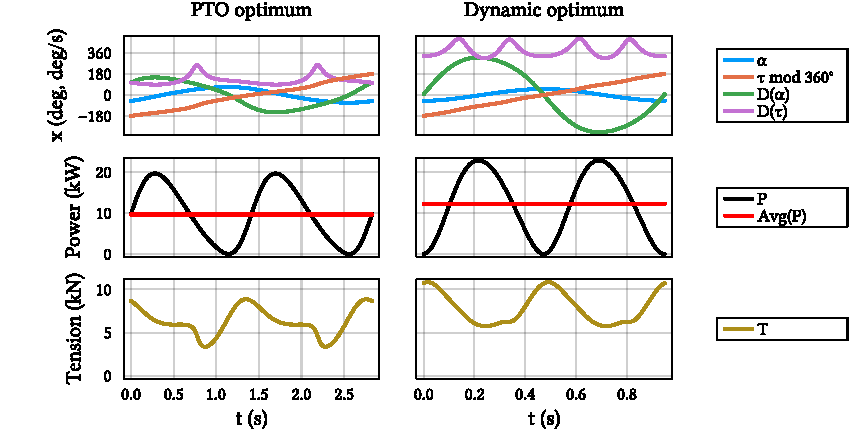
\includegraphics{figs/optimization_timeseries_all.pdf}
    \caption{Limit cycles for the initial guess (PTO optimum, left) and the optimized parameters (dynamic optimum, right): angles and angular velocities (top), instantaneous and average power (middle), line tension (bottom).
    The period goes from \SI{\PeriodInit}{\second} to \SI{\PeriodOpt}{\second}, and the average power increases by \(\PowerGain\%\).}
    \label{fig:time_series}
\end{figure}

\subsection{Optimal design as a function of wind speed} \label{sec:opt-wind}

Since the optimization converges quickly, we repeat the procedure for a range of reference wind speeds \(w_0\).
For each integer wind speed from \SIrange{\SweepWindMin}{\SweepWindMax}{\meter\per\second}, we find the set of parameters (Figure~\ref{fig:parameterized_optimization_params}) that maximizes power (Figure~\ref{fig:parameterized_optimization_power}) and show the corresponding minimum and maximum line tension over the limit cycle (Figure~\ref{fig:parameterized_optimization_tension}).
For comparison, we also compute the power and line tension extrema using the set of parameters obtained in Section~\ref{sec:opt-power}, optimized for a wind speed of \SI{\WindRef}{\meter\per\second}.
Over this whole range, this fixed set of parameters yields at most \(\SweepMaxLoss\%\) less power than the actual optimum, with a maximum line tension at most \(\SweepMaxTensionIncrease\%\) higher.
%\alter{landscape of the objective around the optimum: no asymmetry, just aim for the middle?}
The system exhibits quasilinear scaling along this parameterized optimization, even though the length of the arm (and other parameters) is kept constant, which makes it impossible to scale the model perfectly to wind speed.
Least-squares power laws along the optimized sweep give the following trends:
\begin{itemize}
    \item the average power grows like \(w_0^{\ExpPower}\), to be compared with the \(w_0^3\) scaling of wind power;
    \item the maximum line tension grows like \(w_0^{\ExpTension}\);
    \item the line length \(\ell\) and the arm inertia \(I\) vary as shown in Figure~\ref{fig:parameterized_optimization_params};
    \item the arm braking coefficient \(b\) grows like \(w_0^{\ExpBrake}\);
    \item (not shown) the period varies like \(w_0^{\ExpPeriod}\).
\end{itemize}

The maximum line tension defines the strength requirements for the kite fabric and lines.
Furthermore, the minimum line tension remains above \SI{\SweepMinTension}{\kilo\newton} over the whole sweep, confirming \emph{a posteriori} the modeling assumption that the lines are always in tension and never exert compression on the arm.

\begin{figure}[thpb]
  \centering
  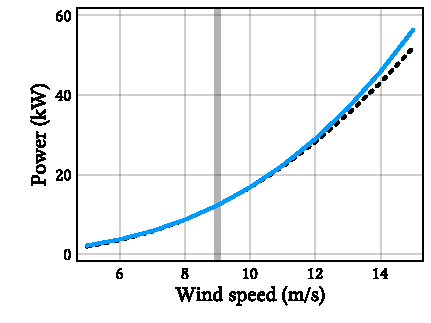
\includegraphics{figs/optimization_wind_sweep_power.pdf}
  \caption{Average generated power for optimized (blue) and reference (black) parameters when the reference wind speed \(w_0\) is varied.
  The reference curve is generated by fixing the design parameters to the optimal values for \(w_0 = \SI{\WindRef}{\meter\per\second}\).}
  \label{fig:parameterized_optimization_power}
\end{figure}

\begin{figure}[thpb]
  \centering
  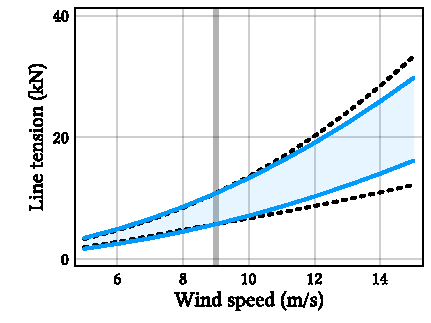
\includegraphics{figs/optimization_wind_sweep_tension.pdf}
  \caption{Minimum and maximum line tension \(\vb F_\ell\) for optimized (blue) and reference (black) parameters.}
  \label{fig:parameterized_optimization_tension}
\end{figure}

\begin{figure}[thpb]
  \centering
  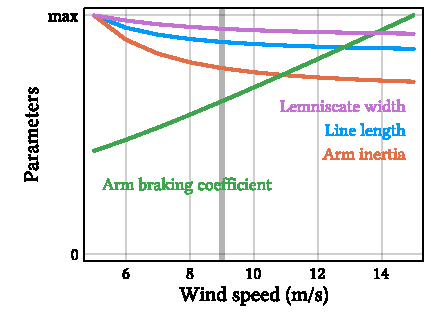
\includegraphics{figs/optimization_wind_sweep_params.pdf}
  \caption{Optimal parameters for each wind speed (color) and reference parameters fixed at the optimum for \(w_0 = \SI{\WindRef}{\meter\per\second}\) (black dashed lines).}
  % At this level of operation and despite relatively strong changes in the environmental parameter, the braking coefficient of the arm behaves linearly with respect to wind speed.
  \label{fig:parameterized_optimization_params}
\end{figure}

\subsection{Curvature of the kite trajectory} \label{sec:opt-curvature}

Besides power, a design has to be compatible with the flight of the kite: the turns of the curve \(t\mapsto\vb r(t)\) it describes must not be too strong.
We therefore derive upper bounds on the curvature \(\kappa\) of this curve; the computations and proofs are given in Appendix~\ref{app:curv}.

\paragraph{Setting.}
Recall that the kite position is \(\vb r = r\,\vu r(\tau)\), where \(\vu r\) is the spherical eight \eqref{eq:sphere_Model_Deriv}--\eqref{eq:traject_Model_Deriv}, a closed curve on the unit sphere with \(0<\theta_0-\Delta\theta\) and \(\theta_0+\Delta\theta<\pi\), and where \(r\) solves the line-length constraint:
\begin{equation}
    r = p + \sqrt{p^2+\ell^2-a^2}, \qquad p = a\,g, \qquad g = \sin\theta\cos(\phi-\alpha),
\end{equation}
so that \(\ell-a\le r\le\ell+a\), and \(r\equiv\ell\) when \(a=0\).
We write \(\varepsilon = a/\ell\) and \(\varepsilon' = a/\sqrt{\ell^2-a^2}\).
The kite trajectory is drawn on the \emph{cone} \(\mathscr C = \{r\,\vu r(\tau) : r>0,\ \tau\in\mathbf{S}^1\}\), the conical hull of the spherical eight.
Along a periodic orbit with \(\dot\tau\ne0\), the arm angle is a function \(\alpha(\tau)\), and since curvature does not depend on the parametrisation, the curvature \(\kappa = \norm{\vb r'\times\vb r''}/\norm{\vb r'}^3\) of the space curve (prime \(=\dv*{}{\tau}\)) does not depend on the time law \(\tau(t)\): \(\kappa(t) = \kappa(\tau(t))\).
It depends on \(\ell\), \(\Delta\theta\), \(\Delta\phi\), \(\theta_0\), \(a\), and on the arm law through \(\alpha,\alpha',\alpha''\); for \(a=0\), only on \(\ell,\Delta\theta,\Delta\phi,\theta_0\).

\paragraph{Curvature formula.}
Let \(v = \norm{\vu r'}\) be the speed on the sphere,
\begin{equation}
    v^2 = 4\Delta\theta^2\cos^22\tau + \Delta\phi^2\sin^2\theta\cos^2\tau > 0,
\end{equation}
\(\sigma(\tau) = \int_0^\tau v\) its arclength (so that \(f_\sigma = f'/v\) and \(f_{\sigma\sigma} = (f''v-f'v')/v^3\) for any function \(f\) of \(\tau\)), \(\vu t = \vu r_\sigma\) its unit tangent, \(\vu n = \vu r\times\vu t\), and \(\kappa_g\) its geodesic curvature on the sphere, defined by \(\vu t_\sigma = -\vu r + \kappa_g\vu n\):
\begin{equation} \label{eq:curv-kg}
    \kappa_g = \frac{2\Delta\theta\Delta\phi\sin\theta\,\sin\tau\,(2+\cos2\tau) + \Delta\phi\cos\theta\cos\tau\,\bigl(8\Delta\theta^2\cos^22\tau + \Delta\phi^2\sin^2\theta\cos^2\tau\bigr)}{v^3}.
\end{equation}
Finally let \(u = \ln r\).
For every \(\tau\),
\begin{equation} \label{eq:curv-formula}
    r\,\kappa = \frac{\sqrt{\kappa_g^2\,(1+u_\sigma^2) + (1+u_\sigma^2-u_{\sigma\sigma})^2}}{(1+u_\sigma^2)^{3/2}}.
\end{equation}
The cone \(\mathscr C\) is a developable surface, with principal curvatures \(0\) along the generators and \(\kappa_g/r\) across them.
Formula \eqref{eq:curv-formula} is the decomposition \(\kappa^2 = \kappa_n^2 + (\kappa_g^{\mathscr C})^2\) of the curvature of a curve drawn on \(\mathscr C\) into its normal and geodesic parts:
\begin{equation}
    \kappa_n = \frac{\kappa_g}{r}\sin^2\beta = \frac{\kappa_g}{r\,(1+u_\sigma^2)}, \qquad \kappa_g^{\mathscr C} = \frac{1+u_\sigma^2-u_{\sigma\sigma}}{r\,(1+u_\sigma^2)^{3/2}},
\end{equation}
where \(\beta\) is the angle between the trajectory and the generator.
The normal part is controlled by the curvature of the surface, \(\abs{\kappa_n}\le\abs{\kappa_g}/r\), and is entirely due to the bending of the spherical eight; the geodesic part is the curvature of the planar polar curve \(\sigma\mapsto r(\sigma)\) obtained by unrolling the cone, and is due to the variation of \(r=\norm{\vb r}\) along the cycle.
The surface therefore bounds \(\kappa\) from below only, by \(\abs{\kappa_n}\); this lower bound vanishes at the inflection points of the eight, where \(\kappa_g=0\), and it gives no upper bound.

\paragraph{Without arm.}
For \(a=0\), the trajectory lies on the sphere of radius \(\ell\), the unrolled curve is a circle of radius \(\ell\), and
\begin{equation}
    \kappa = \frac{\sqrt{1+\kappa_g^2}}{\ell} \ \ge\ \frac1\ell,
\end{equation}
with equality at the inflection points of the eight, which exist on each lobe.
In particular, the floor \(1/\ell\) is a property of the trajectory in the cone, not of the cone.
Large curvature is produced where the spherical eight turns sharply, \emph{i.e.} where \(v\) is small compared with the bending of the eight: at the lobe tips \(\tau=\pi/2,3\pi/2\) for a wide eight (\(\Delta\theta\) small compared with \(\Delta\phi\sin\theta_0\)), and at the top and bottom \(\tau=\pi/4,3\pi/4\) for a tall eight.
Indeed, exactly,
\begin{equation}
    \kappa_g(\pi/2) = \frac{\Delta\phi\sin\theta_0}{4\Delta\theta^2}, \qquad
    \kappa_g(3\pi/4) = \frac{8\Delta\theta}{\Delta\phi^2\sin^2(\theta_0-\Delta\theta)} - \cot(\theta_0-\Delta\theta),
\end{equation}
so that, for \(a=0\), \(\max\kappa\to\infty\) as \(\Delta\theta\to0\) or as \(\Delta\phi\to0\), the other parameters being fixed.

\paragraph{Upper bound.}
Consider a box of parameters: let \(\ell\ge\ell_->a\), \(\Delta\theta\in[\Delta\theta_-,\Delta\theta_+]\), \(\Delta\phi\in[\Delta\phi_-,\Delta\phi_+]\) with \(\Delta\theta_->0\), \(\Delta\phi_->0\), and \(\theta_0\in[\theta_{0-},\theta_{0+}]\) with \(\mathscr J = [\theta_{0-}-\Delta\theta_+,\ \theta_{0+}+\Delta\theta_+]\subset(0,\pi)\).
Set
\begin{equation}
    m = \min_{\mathscr J}\sin, \qquad M = \max_{\mathscr J}\sin, \qquad C = \max_{\mathscr J}\abs{\cos},
\end{equation}
\begin{equation}
    v_* = \begin{cases}
        2\Delta\theta_- & \text{if } m\Delta\phi_-\ge4\Delta\theta_-, \\[2pt]
        m\Delta\phi_-\sqrt{\dfrac12 - \dfrac{m^2\Delta\phi_-^2}{64\,\Delta\theta_-^2}} & \text{otherwise,}
    \end{cases}
    \qquad
    \bar\kappa_g = \frac{2\sqrt2\,M\,\Delta\theta_+\Delta\phi_+}{v_*^3} + \frac{2C}{m}.
\end{equation}
Let the arm law satisfy \(\abs{\alpha'}\le A_1\) and \(\abs{\alpha''}\le A_2\), and set
\begin{equation}
\begin{split}
    &\Gamma_1 = 2\Delta\theta_+ + \Delta\phi_+ + A_1, \qquad \Gamma_2 = \Gamma_1^2 + 4\Delta\theta_+ + \Delta\phi_+ + A_2, \\
    &V_1 = 4\Delta\theta_+ + \Delta\phi_+ + \tfrac12\Delta\phi_+^2 + 4\Delta\theta_+\Delta\phi_+, \qquad
    U = \varepsilon'\,\frac{\Gamma_2 + \varepsilon'^2\,\Gamma_1^2}{v_*^2} + \varepsilon'\,\frac{\Gamma_1V_1}{v_*^3}.
\end{split}
\end{equation}
Then, for all parameters in the box, every such arm law, and every \(\tau\),
\begin{equation} \label{eq:curv-bound}
    \kappa \le \frac{\sqrt{\bar\kappa_g^2 + (1+U)^2}}{\ell_--a},
\end{equation}
and, without arm (\(a=0\), \(U=0\)), \(1/\ell\le\kappa\le\sqrt{1+\bar\kappa_g^2}/\ell_-\).
Since \(U = O(\varepsilon)\), the bound is \(\sqrt{1+\bar\kappa_g^2}/\ell_- + O(\varepsilon)\), uniformly on the box.
The bound degenerates only when \(\Delta\theta_-\to0\), \(\Delta\phi_-\to0\), or \(\mathscr J\) reaches a pole, which is unavoidable by the exact tip and bottom values above; and, when \(a>0\), the bound on \(\alpha''\) cannot be dispensed with, since \(u_{\sigma\sigma}\), which contains \(\alpha''\) linearly, enters \eqref{eq:curv-formula} through \(\abs{1+u_\sigma^2-u_{\sigma\sigma}}\).
In the optimization above, the lower bound on \(\ell\) in Table~\ref{tab:opt_descr} plays the role of \(\ell_-\), while \(A_1\) and \(A_2\) can be evaluated on the computed periodic orbits.

\paragraph{First order in the arm length.}
With \(K = \sqrt{1+\kappa_g^2}\), for a fixed eight and a fixed arm law with bounded \(\alpha',\alpha''\),
\begin{equation} \label{eq:curv-first-order}
    \ell\,\kappa = K\,(1-\varepsilon g) - \varepsilon\,\frac{g_{\sigma\sigma}}{K} + O(\varepsilon^2)
\end{equation}
uniformly in \(\tau\): the arm rescales the arm-free curvature by \(\ell/r\) and adds the contribution of the second derivative of \(g\) (hence of \(\alpha''\)) along the eight.

\paragraph{Example (without arm).}
For the optimized eight of Table~\ref{tab:opt_results} (\(\Delta\theta=\DthetaFixed^\circ\), \(\Delta\phi=\DphiOpt^\circ\), \(\theta_0=\ThetaZero^\circ\)), the exact value above gives \(\kappa_g(\pi/2)\simeq\CurvTipKg\), hence \(\ell\kappa(\pi/2) = \sqrt{1+\kappa_g(\pi/2)^2} \simeq \CurvTipK\) at the lobe tips for \(a=0\).
This value at the tip is exact: it follows from the formulas above, with no approximation.
The tips are not necessarily where the turn is sharpest: sampling \(\tau\) on a fine grid gives \(\max_\tau\ell\kappa\simeq\CurvMaxK\), reached at \(\tau\simeq\CurvMaxTau\) and, by symmetry, at \(\tau+\pi\); the smallest radius of curvature of the trajectory is thus about \(\ell/\CurvMaxK\), \emph{i.e.} about \SI{\CurvMaxRadius}{\meter} for the optimized length \(\ell=\SI{\EllOpt}{\meter}\).
The case \(a>0\) was not examined here; there, only the upper bound \eqref{eq:curv-bound} is proven.


\begin{table}[htbp]
  \centering
  \caption{Comparison of initial and optimized parameters}
  \label{tab:parameter_comparison}
  \begin{tabular}{lrr}
    \toprule
    Parameter & \multicolumn{1}{c}{PTO initialization} & \multicolumn{1}{c}{Dynamic ptimization} \\
    \midrule
    $\ell$ ($\mathrm{m}$)                             & 31.0     & 26.9679  \\
    $I$ ($\mathrm{kg\cdot m^2}$)                     & 1300.0   & 351.628  \\
    $b$ ($\mathrm{kg\cdot m^2\cdot s^{-1}\cdot rad^{-1}}$) & 2888.29  & 737.073  \\
    $\Delta\phi$ ($\mathrm{rad}$)                    & 0.872665 & 0.29     \\
    \midrule
    Period ($\mathrm{s}$)                            & 2.82807  & 0.949268 \\
    Objective $P$ ($\mathrm{kW}$)                    & 9.63887  & 12.2534  \\
    Min tension ($\mathrm{kN}$)                      & 3.35552  & 5.74767  \\
    Max tension ($\mathrm{kN}$)                      & 8.85567  & 10.8269  \\
    Max acceleration ($\mathrm{m/s^2}$)              & 517.078  & 938.602  \\
    \bottomrule
  \end{tabular}
\end{table}



\begin{figure}[thpb]
    \centering
        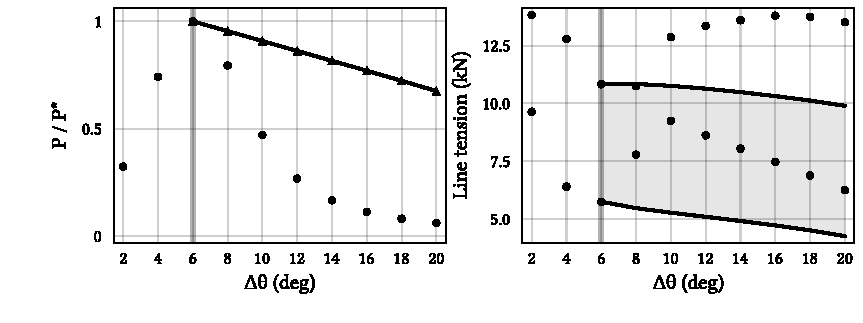
\includegraphics{figs/optimization_dtheta.pdf}
    \caption{Average power and line tension and acceleration as $\Delta \theta$ varies. 6° gives a good combination of average power (higher is better) and line tension (lower is better).}
    \label{fig:opt-dtheta}
\end{figure}

\begin{figure}[thpb]
    \centering
    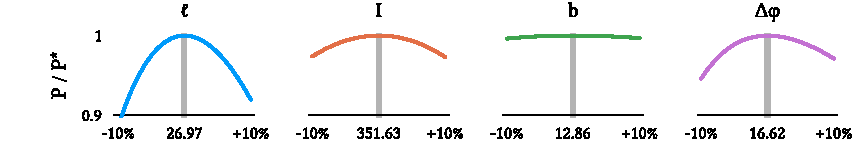
\includegraphics{figs/optimization_landscape.pdf}
    \caption{Average power as the optimization parameters vary.
    % TODO which variables are on their bounds? which variables have the most impact? could reoptimize other 3 parameters
    The objective landscape is smooth, explaining the easy numerical solving.}
    \label{fig:opt-landscape}
\end{figure}


\appendix

\section{10D model} \label{sec:model10D}
\subsection{Model description}
% TODO cite Fagiano PhD thesis and Diehl PhD thesis
In this appendix, we describe the model designed by Alain Nême inspired by Fagiano PhD thesis and Diehl PhD thesis. 
The objective is to have an ODE that does not involve a control to simulate a kite flying horizontal eights, or lemniscates, while the arm extracts energy from the system.
The kite $K$ is attached to the tip of a rotating arm $A$ of length $a$ with four lines of length $\ell$ (assumed constant), the arm rotates around $\vu z$ at the origin $O$.

\subsection{Static and kinematics}
Let us define three unit vectors: $\vu a$ follows the arm, $\hat{\boldsymbol{\ell}}$ follows the lines and $\vu r$ points to the kite:
\begin{align}
    \vu a &= \frac{\vb a}{\norm{\vb a}} = \begin{pmatrix}
        \cos(\alpha) \\ \sin(\alpha) \\ 0
    \end{pmatrix} \\
    \hat{\boldsymbol{\ell}} &= \frac{\boldsymbol{\ell}}{\norm{\boldsymbol{\ell}}} = \begin{pmatrix}
        \sin(\theta_\ell) \cos(\alpha + \phi_\ell) \\ \sin(\theta_\ell) \sin(\alpha + \phi_\ell) \\ \cos(\theta_\ell)
    \end{pmatrix} \\ \label{eq:that-10D}
    \vu r &= \frac{\vb r}{\norm{\vb r}} = \begin{pmatrix}
        \sin(\theta(\tau)) \cos(\phi(\tau)) \\ \sin(\theta(\tau)) \sin(\phi(\tau)) \\ \cos(\theta(\tau))
    \end{pmatrix} \text{ with}
    \begin{cases}
        \theta : \tau \mapsto \theta_0 + \Delta \theta \sin(2\tau) \\
        \phi : \tau \mapsto \Delta \phi \sin(\tau)
    \end{cases}.
\end{align}
%
Here, $\alpha$ is the angle between the arm and the $x$-axis (aligned with the wind), $\theta_\ell$, $\phi_\ell$ are the spherical coordinates of $K$ in $(A, \vu a, \vu z \times \vu a, \vu z)$, and $R$, $\theta$ and $\phi$ are the spherical coordinates of $K$ in $(O, \vu x, \vu y, \vu z)$.
Spherical coordinates use the physics convention also found in ISO 80000-2:2019:
\begin{itemize}
    \item $R$ is the radius,
    \item $\theta$ is the polar angle from the $z$-axis,
    \item $\phi$ is the azimuthal angle from the $x$-axis.
\end{itemize}
%
% TODO Spherical coordinates in annex with more details and a figure?
The state of the system at time $t$ is given by the configuration vector
\begin{equation} \label{eq:state_vector}
    \vq(t) = (\alpha(t), \theta_\ell(t), \phi_\ell(t), R(t), \tau(t))
\end{equation}
%
and its corresponding velocities $\dq(t)$, while $\theta_0$, $\Delta \theta$ and $\Delta \phi$ are the parameters that control the shape of the lemniscate.
Note that:
\begin{itemize}
    \item $\vb a$ depends only on state $\alpha$,
    \item $\boldsymbol{\ell}$ depends only on state $\theta_\ell$ and $\phi_\ell$,
    \item $\vb r$ depends only on state $R$ and $\tau$.
\end{itemize}
%
Using Chasles' relation, we get the following loop closure condition:
\begin{equation} \label{eq:loop_closure_vector}
    \vb r = \vb a + \boldsymbol{\ell}.
\end{equation}
%
We define
\begin{equation} \label{eq:func_g}
\begin{split}
    \vb g : \vq \in \R^5 \mapsto
    \vb g(\vq) &= \vb r(\vq) - \vb a(\vq) - \boldsymbol{\ell}(\vq) \\
    &= \begin{pmatrix}
        R \sin(\theta(\tau)) \cos(\phi(\tau)) - a \cos(\alpha) - \ell \sin(\theta_\ell) \cos(\alpha + \phi_\ell) \\
        R \sin(\theta(\tau)) \sin(\phi(\tau)) - a \sin(\alpha) - \ell \sin(\theta_\ell) \sin(\alpha + \phi_\ell) \\
        R \cos(\theta(\tau)) - \ell \cos(\theta_\ell)
    \end{pmatrix} \in \R^3
\end{split}
\end{equation}
such that \eqref{eq:loop_closure_vector} rewrites to
\begin{equation} \label{eq:loop_closure_function}
    \vb g(\vq) = 0_{\R^3}
\end{equation}
We have a five dimensional state (\emph{cf.} \ref{eq:state_vector}) subject to three algebraic constraints (\emph{cf.} \ref{eq:loop_closure_function}), thus the system has two \ac{dof}.

\begin{remark} 
The set of acceptable positions for $K$ is the intersection between a filled torus (filled \emph{spindle} torus if the lines are longer than the arm, \emph{i.e.} $\ell > a$) and an eight-shaped cone.
See Fig.~\ref{fig:spindle_torus} and Section~\ref{sec:model-geometry}.
\end{remark}

\subsection{Dynamics}  \label{sec:model10D-dynamics}

We assume that all forces apply to the kite at point $K$ of mass $m$ and all moments apply to the arm which rotates around $\vu z$ at point $O$.
We want to determine $\ddq$ in terms of $\vq$ and $\dq$.

% \subsubsection*{Aerodynamic forces}
\label{sec:model10D-dyn-aero}

We choose the 1/7-power-law profile to model the wind, such that the wind speed $\vb w$ at altitude $z$ is given by $\vb w(z) = w_r \qty( z / z_r )^{1/7} \vu x$.
The apparent wind, the wind which is felt by the kite, is then $\vb w_a = \vb w - \dot{\vb r}$.
The lift $L$ and drag $D$ of the kite are respectively
\begin{align}
    L &= \frac{1}{2} S \rho_a C_L \norm{\vb w_a}^2 \\
    D &= \frac{1}{2} S \rho_a C_D \norm{\vb w_a}^2
\end{align}
%
where $S$ is the surface of the kite, $\rho_a$ is the density of the air and $C_L$ and $C_D$ the lift and drag coefficients.
Using the lift-to-drag ratio $f = L / D$, we get the simpler $D = L/f$.
realistically, $C_L$ and $C_D$ should depend on the angle of incidence, but we don't model this angle and assume of value of $0$.
To determine the direction of the lift and drag forces, we assume that the chord of the kite is aligned with the apparent wind, and that its leading edge is perpendicular to the lines, which completely determines the orientation of the kite.
Let us define $\vu k_b$ the unit vector aligned with the chord pointing to the \emph{back} of the kite, $\vu k_r$ the unit vector aligned with the leading edge pointing to the \emph{right} of the kite, and $\vu k_t$ the unit vector normal to the surface of the kite pointing to its \emph{top}.
We have :
\begin{align}
    \vu k_b &= \frac{\vb w_a }{\norm{\vb w_a}} \\
    \vu k_r &= \frac{\hat{\boldsymbol{\ell}} \times \vu k_b}{\norm{\hat{\boldsymbol{\ell}} \times \vu k_b}} \\
    \vu k_t &= \vu k_b \times \vu k_r.
\end{align}
We then obtain the aerodynamic forces of the kite
\begin{align}
    \vb L &= L \vu k_t \\
    \vb D &= D \vu k_b.
\end{align}

% TODO SCHEMA pour top bottom right dans la perspective du kite

To assess the impact of line length on the performance of the device, we also need to model the drag of the lines.
Let us first define the apparent wind of the lines at distance $\lambda$ from the attachment point $A$:
\begin{equation}
    \vb w_{a,\ell}(\lambda) = \vb w\qty(\frac{\lambda}{\ell} K_z) - \frac{\lambda}{\ell} \dot{\vb r} - \qty(1 - \frac{\lambda}{\ell}) \dot{\vb a},
\end{equation}
%
and $\vu w_a = \frac{\vb w_a}{\norm{\vb w_a}}$ is its unit vector.
Let \(\theta_a\) be the angle between the lines and the apparent wind: \(\hat{\boldsymbol{\ell}} \cdot \vu w_{a,\ell} = \cos(\theta_a)\), so that \(\sin(\theta_a) = \sqrt{1 - (\hat{\boldsymbol{\ell}} \cdot \vu w_{a,\ell})^2}\).
% QUESTION (PR #78, abavoil): projected area (drag in sin theta_a) or cross-flow principle (sin^2 theta_a)? The code (PointMass4._forces) uses the cross-flow form below.
Following the cross-flow principle, the drag of an element of line of length \(\dd{\lambda}\) and diameter \(d_\ell\) depends only on the component of the apparent wind orthogonal to the lines, \(\vb w_{a,\ell}^\perp = \vb w_{a,\ell} - (\hat{\boldsymbol{\ell}} \cdot \vb w_{a,\ell})\,\hat{\boldsymbol{\ell}}\), of norm \(\norm{\vb w_{a,\ell}}\sin(\theta_a)\), and is directed along it.
The drag of the \(n = 4\) lines with drag coefficient \(C_{D,\ell}\) is
\begin{equation}
    \vb D_\ell
    = \bigintssss \limits_{\lambda = 0}^{\lambda = \ell} \frac{1}{2} n d_\ell \rho_a C_{D,\ell} \norm{\vb w_{a,\ell}^\perp(\lambda)}\, \vb w_{a,\ell}^\perp(\lambda) \dd{\lambda}
    = \frac{1}{2} n \ell d_\ell \rho_a C_{D,\ell} \int \limits_{\xi=0}^{\xi=1} \norm{\vb w_{a,\ell}^\perp(\ell \xi)}\, \vb w_{a,\ell}^\perp(\ell \xi) \dd{\xi}.
\end{equation}
%
We approximate this integral by assuming that the speed of \(A\) is negligible, \(\dot{\vb a} \approx 0\), and that the apparent wind varies linearly along the lines, \(\vb w_{a,\ell}(\ell\xi) \approx \xi\, \vb w_a\).
Then \(\vb w_{a,\ell}^\perp(\ell\xi) \approx \xi\, \vb w_a^\perp\), and the integral of \(\xi^2\) over \([0,1]\) gives the approximated drag of the lines
\begin{equation} \label{eq:line-drag-10D}
    \tilde{\vb D}_\ell = \tilde D_\ell\, \vu w_a^\perp, \qquad \tilde D_\ell = \frac{1}{6} n \ell d_\ell \rho_a C_{D,\ell} \norm{\vb w_a^\perp}^2, \qquad \vu w_a^\perp = \frac{\vb w_a^\perp}{\norm{\vb w_a^\perp}},
\end{equation}
and the total aerodynamic force of the system is
\begin{equation} \label{eq:f_aero_10D}
    \vb F_a = L \vu k_t + D \vu k_b + \tilde D_\ell \vu w_a^\perp.
\end{equation}
In all the computations of this paper, \(C_{D,\ell} = 0\): the drag of the lines is lumped into the drag coefficient \(C_D\) of the kite.
% \subsubsection*{Gravity}

The kite has mass $m$ and the lines have density $\rho_\ell$, therefore their mass is $m_\ell = n \pi \ell \rho_\ell d_\ell^2 / 4$.
We assume that the kite lifts half of the lines, while the rest is supported by the arm.
The total flying mass is then $m + m_\ell/2$ and the total weight is
\begin{equation} \label{eq:f_grav_10D}
    \vb F_g = -\qty(m + \frac{m_\ell}{2}) g \vu z.
\end{equation}

% \subsubsection*{Line tension and torque on the arm}

We denote $\vb F_\ell = -F_\ell \hat{\boldsymbol{\ell}}$ the tension of the lines on the kite, then, the torque applied by the lines on the arm is
\begin{equation}
    \vb T_\ell = \vb a \times (- \vb F_\ell) = a F_\ell \vu a \times \hat{\boldsymbol{\ell}}.
\end{equation}
%
Since the arm rotates around the $z$ axis, only the torque in the $z$ direction has an effect, therefore we only need the $z$ component of $\vb T_\ell$.
Also, for computing the cross-product, let us rewrite the vectors $\vu a$ and $\hat{\boldsymbol{\ell}}$ in the base attached to the arm $\mathscr B_a = (\vu a, \vu z \times \vu a, \vu z)$; trivially, $\vu a = 1 \vu a$ and 
\begin{equation} \label{eq:lhat-10D}
    \hat{\boldsymbol{\ell}} = \sin(\theta_\ell) \cos(\phi_\ell) \vu a + \sin(\theta_\ell) \sin(\phi_\ell) (\vu z \times \vu a) + \cos(\theta_\ell) \vu z.
\end{equation}
%
Let us now compute the cross-product:
\begin{equation}
    \vu z \cdot (F_\ell \vu a \times \hat{\boldsymbol{\ell}}) = 1 \cdot \sin(\theta_\ell) \sin(\phi_\ell) - 0 \cdot \sin(\theta_\ell) \cos(\phi_\ell) = \sin(\theta_\ell) \sin(\phi_\ell),
\end{equation}
%
from which we finally get the expression for the effective torque of the lines:
\begin{equation}
    \vb T_\ell \cdot \vu z = a F_\ell \sin(\theta_\ell) \sin(\phi_\ell).
\end{equation}
%
The torque of the generator on the arm is $T : \omega \mapsto -b \omega$ where $b$ is a rotational viscous damping coefficient with dimension of torque per angular velocity, and the arm has inertia $I$, such that using Newton's second law, we get
\begin{equation} \label{eq:newton_arm_10D}
    I \ddot \alpha
    = \vb T_\ell \cdot \vu z + T(\dot \alpha)
    = a F_\ell \sin(\theta_\ell) \sin(\phi_\ell) - b \dot \alpha,
\end{equation}
from which we compute $\vb F_\ell$, directed by $-\hat{\boldsymbol{\ell}}$:
\begin{equation} \label{eq:f_lines-10D}
    \vb F_\ell = \frac{-I \ddot \alpha - b \dot \alpha}{a \sin(\theta_\ell) \sin(\phi_\ell)} \hat{\boldsymbol{\ell}}.
\end{equation}
In the above, the lever arm of the tension is $a \sin(\theta_\ell) \sin(\phi_\ell)$. For $\sin(\theta_\ell)$ to be zero, the kite would have to fly underground directly below the tip of the arm, which won't happen, or directly above it, which also won't happen if $\theta_0 - \Delta \theta > 0$, \emph{cf}. \ref{eq:lhat-10D}, which is verified for realistic values of $\theta_0$ and $\Delta \theta$.
% TODO better explanation?
% TODO define when it breaks: when does proj_xy(K) equal A?
With a typical choice of parameters the kite will never fly directly above the tip of the arm, thus $\sin(\theta_\ell) > 0$ at all times.
However, $\sin(\phi_\ell)$ could very well be null, but the singularity is only in the equations, as we observe no exceptional behavior when the lines and the arm are aligned ($xy$-plane); for the reduced model, it is removed by solving the equation of the arm for $\ddot\alpha$ instead of the tension (Section~\ref{sec:model-eom} and Appendix~\ref{sec:explicit-ddq}).

% \subsubsection*{Fictitious force of the cone}
To understand this section better, let's picture a train on a railway.
The train doesn't control where by steering (a \emph{control} in the mathematical sense), instead, the railway exerts a force on the train, always perpendicular to railway/the direction of the train, that keeps the train on the track passively.
We want the eight-shaped cone to play the role of the railway to passively steer the kite into eight-shaped trajectories.
One way to physically describe this interaction is that the kite glides without friction on the manifold, therefore it feels a fictitious force $\vb F_c$ always perpendicular to the manifold.
The cone has two tangent vectors $\pdv{\vb r}{R}$ and $\pdv{\vb r}{\tau}$, therefore it is normal to both:
\begin{equation}\begin{cases} \label{eq:f_cone_constraint_10D}
    \vb F_c \cdot \pdv{\vb r}{R} = 0 \\
    \vb F_c \cdot \pdv{\vb r}{\tau} = 0.
\end{cases}\end{equation}

\subsection{applying Newton's second law to the kite}

Newton's second law applied to the kite's center of mass gives
\begin{equation} \label{eq:newton_kite_10D}
    m \ddot{\vb r} = \vb F_a + \vb F_g + \vb F_\ell + \vb F_c.
\end{equation}
%
At this point, we need to choose two equations to keep, while the others will be used at substitutions.
For their nice symmetry, we keep \ref{eq:f_cone_constraint_10D} and use the others to express $\vb F_c$ in terms of $\vq, \dq$, and $\ddq$.
From \ref{eq:newton_kite_10D}, we have that
\begin{equation} \label{eq:f_cone_newton_10D}
    \vb F_c = m \ddot{\vb r} - \vb F_a - \vb F_g - \vb F_\ell.
\end{equation}
%
The acceleration of the kite $\ddot{\vb r}$ obtained by differentiating twice its position $\vb r$:
\begin{equation}
    \vb r = R \vu r = R \begin{pmatrix}
        \sin(\theta) \cos(\phi) \\
        \sin(\theta) \sin(\phi) \\
        \cos(\theta)
    \end{pmatrix},
\end{equation}
%
\begin{equation}\begin{split}
    \dot{\vb r} &= \dot R \vu r + R \dot{\vu r}
    = \dot R \begin{pmatrix}
        \sin(\theta) \cos(\phi) \\
        \sin(\theta) \sin(\phi) \\
        \cos(\theta)
    \end{pmatrix} + R \begin{pmatrix}
        \cos(\theta) \cos(\phi) \dot \theta - \sin(\theta) \sin(\phi) \dot \phi \\
        \cos(\theta) \sin(\phi) \dot \theta + \sin(\theta) \cos(\phi) \dot \phi \\
        -\sin(\theta) \dot \theta
    \end{pmatrix} \\
    &= \begin{pmatrix}
        \sin(\theta) \cos(\phi) \dot R + \cos(\theta) \cos(\phi) \dot \theta - \sin(\theta) \sin(\phi) \dot \phi \\
        \sin(\theta) \sin(\phi) \dot R + \cos(\theta) \sin(\phi) \dot \theta + \sin(\theta) \cos(\phi) \dot \phi \\
        \cos(\theta) \dot R - \sin(\theta) \dot \theta
    \end{pmatrix},
\end{split}\end{equation}
%
\begin{equation}\begin{split}
    \ddot{\vb r} &= \ddot R \vu r + \dot R \dot{\vu r} + \dot R \dot{\vu r} + R \ddot{\vu r} = \ddot R \vu r + 2 \dot R \dot{\vu r} + R \ddot{\vu r}.
\end{split}\end{equation}
%
% TODO continue developing to have the full expression of ddot OK?
%
The three forces $\vb F_g$, $\vb F_a(\vq, \dq)$, and a$\vb F_\ell(\vq, \dq, \ddq)$ are developed in \ref{eq:f_grav_10D}, \ref{eq:f_aero_10D}, and \ref{eq:f_lines-10D} respectively.

We have written every quantity in \ref{eq:f_cone_newton_10D} explicitly in terms of $\vq$, $\dq$, and $\ddq$, thus \ref{eq:f_cone_constraint_10D} is a system of two second order \ac{ode}s in $\vq \in \R^5$.
By combining \ref{eq:f_cone_constraint_10D} and \ref{eq:loop_closure_function}, we obtain the following system of two implicit second order \ac{ode}s and three algebraic equations (or constraints):
%
\begin{equation}\begin{cases}
    \vb F_c(\vq, \dq, \ddq) \cdot {\pdv{\vb r}{R}}(\vq) = 0 \\
    \vb F_c(\vq, \dq, \ddq) \cdot {\pdv{\vb r}{\tau}}(\vq) = 0 \\
    R \sin(\theta(\tau)) \cos(\phi(\tau)) - a \cos(\alpha) - \ell \sin(\theta_\ell) \cos(\alpha + \phi_\ell) = 0 \\
    R \sin(\theta(\tau)) \sin(\phi(\tau)) - a \sin(\alpha) - \ell \sin(\theta_\ell) \sin(\alpha + \phi_\ell) = 0 \\
    R \cos(\theta(\tau)) - \ell \cos(\theta_\ell) = 0,
\end{cases}\end{equation}
%
which can be rewritten as
%
\begin{equation}\begin{cases} \label{eq:dae}
    \vb f(\vq, \dq, \ddq) &= 0_{\R^2} \\
    \vb g(\vq) &= 0_{\R^3},
\end{cases}\end{equation}
%
with
%
\begin{equation}
    \vb f(\vq, \dq, \ddq) = \begin{pmatrix}
        \vb F_c(\vq, \dq, \ddq) \cdot {\pdv{\vb r}{R}}(\vq) \\
        \vb F_c(\vq, \dq, \ddq) \cdot {\pdv{\vb r}{\tau}}(\vq)
    \end{pmatrix}
\end{equation}

\subsection{Numerical solving}
The system found in \ref{eq:dae} consists of two \ac{ode}s and three algebraic equations of $\vq : t \mapsto \vq(t) \in \R^5$, therefore it is a \ac{dae}.
The first step toward a solution is to reduce it to a system of \ac{ode}s, which is called index reduction.
It consists in differentiating the algebraic equations with respect to time until we have a system of \ac{ode}s, while adding initial conditions to keep the original algebraic equations valid at all times.
The algebraic equation $\vb g(\vq) = 0$ is reduced to
\begin{equation}\begin{cases} \dg(\vq, \dq) = 0 \\ \vb g(\vq(t_0)) = 0,\end{cases}\end{equation}
and differentiating a second time yields
\begin{equation}\begin{cases} \ddg(\vq, \dq, \ddq) = 0 \\ \dg(\vq(t_0), \dq(t_0)) = 0 \\ \vb g(\vq(t_0)) = 0,\end{cases}\end{equation}
which also exhibits three new algebraic equations that were previously hidden: $\dg(\vq, \dq) = 0$, \emph{i.e.} not only must the configuration be consistent, but the velocities as well.
% TODO Show the differentiation of g?
In our particular case, \emph{two} differentiation steps are required, thus we are working with an \emph{index $2$} \ac{dae}.
By doing so, our system is reduced to $5$ second order \ac{ode}s and $6$ initial conditions:
\begin{equation}\begin{cases}
    \vb f(\vq, \dq, \ddq) = 0_{\R^2} \\
    \ddg(\vq, \dq, \ddq) = 0_{\R^3} \\
    \dg(\vq(t_0), \dq(t_0)) = 0_{\R^3} \\
    \vb g(\vq(t_0)) = 0_{\R^3},
\end{cases}\end{equation}
We introduce $v = \dq$ and rewrite this previous system with only first order \ac{ode}s and initial conditions:
\begin{equation}\begin{cases}
    \vb f(\vq, \vb v, \dot{\vb v}) = 0_{\R^2} \\
    \ddg(\vq, \vb v, \dot{\vb v}) = 0_{\R^3} \\
    \dq - \vb v = 0_{\R^5} \\
    \dg(\vq(t_0), \vb v(t_0)) = 0_{\R^3} \\
    \vb g(\vq(t_0)) = 0_{\R^3}.
\end{cases}\end{equation}
The first two vector equations are implicit and affine in $\dot{\vb v}$: we use a symbolic solver to solve them and have the explicit expression of $\dot{\vb v}$ directly written into our code.
As for the initialization, we have to choose $(\vq, \vb v) \in \R^{5+5}$ verifying the six implicit nonlinear constraints.
To make the solving easier, we set
\begin{equation}\begin{cases}
    \alpha(t_0) = 0 \\
    \dot \alpha(t_0) = 0,
\end{cases}\end{equation}
and let the user choose $(\tau(t_0), \dot \tau) \in \R^2$.
We again use a symbolic solver to determine the rest of the initial conditions as a function of $(\tau(t_0), \dot \tau(t_0))$.

We can finally solve the system numerically using an \ac{ode} solver like Runge-Kutta 5(4) to get the trajectory shown on the left pane of Fig.~\ref{fig:traj-10D}.

On the left pane, over a short horizon, $\vb a + \boldsymbol{\ell}$ seems to coincide with $\vb r$; yet on the middle pane, by integrating for longer, the two trajectories diverge.
Even though we initialize such that $\dg(\vq(t_0)) = 0$ and the \ac{ode} part enforces $\ddg(\vq, \vb v, \dot{\vb v}) = 0$, the slight integration error made at each time step accumulate and make $\dg$, and eventually $\vb g$, drift away from zero (Fig.~\ref{fig:residuals-10D}).
% TODO runtime

\subsection{Limitations of this approach}
% TODO Is this better written? -- We knowingly pick a loose tolerance to exacerbate the problem: even with a correct initialization, the algebraic residuals accumulate an error over time, so much so that after 80 seconds, the state is completely incoherent, \(r, \tau\) and \(\alpha, \theta_l, \phi_l\) telling completely different stories about the position of the kite $K$. For this reason, we introduce a \emph{manifold projection callback}: after every Runge-Kutta step, we apply a Newton algorithm on the state.}

We just saw that the method in not stable for longer integration periods.

% TODO cite diffeqcallback.jl
This can be avoided by using a callback to project $(\vq, \vb v)$ on the acceptable manifold
\begin{equation}
    \left\{ (\vq, \vb v) \in \R^{5+5} \mid \vb g(\vq) = 0 \land \dg(\vq, \vb v) = 0 \right\}
\end{equation}
using one or multiple steps of Newton's method.
The state then stays coherent at all times (right pane of Fig.~\ref{fig:traj-10D}, and Fig.~\ref{fig:residuals-10D}) but the running time is multiplied by two.
% TODO table of run times? at least give some values
Another limitation of this approach include the reliance on an external symbolic solver, whose output is copy pasted into the code, therefore the code is unreadable and hard to maintain, and a small change in the model requires re-running the symbolic solver.

\begin{figure}[thpb]
    \centering
    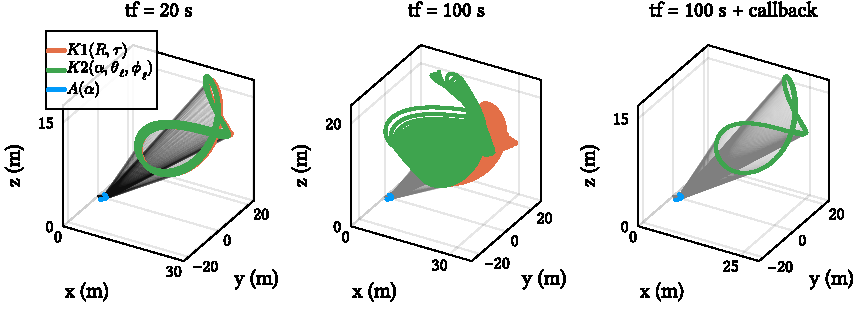
\includegraphics[width=\textwidth]{figs/trajectory_10D_short_long_cb}
    \caption{Kite trajectory of the 10D model integrated with a loose tolerance: short horizon (left), long horizon (middle), long horizon with the manifold projection callback (right).
    Without the callback, the positions given by $\vb r$ and by $\vb a + \boldsymbol{\ell}$ drift apart.}
    \label{fig:traj-10D}
    % web-code: src/numerics_10d.jl#setup_10d src/numerics_10d.jl#traj_10d
\end{figure}

\begin{figure}[thpb]
    \centering
    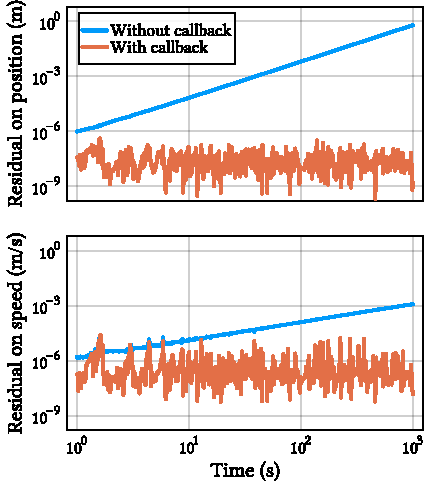
\includegraphics{figs/residuals_10D_interp}
    \caption{Residuals of the configuration constraints of the 10D model on position (top) and on velocity (bottom) along the trajectory, without and with the manifold projection callback.}
    \label{fig:residuals-10D}
    % web-code: src/numerics_10d.jl#setup_10d src/numerics_10d.jl#residuals_10d
\end{figure}

As previously mentioned, this model has five states but only two degrees of freedom; this observation motivates the main result of the paper, which is a whole rewrite of the model by having only two states and no configuration constraint.
The pure \ac{ode} form makes the analytical work much easier, the numerical solution has no drift and is computed much faster because of the reduced number of dimensions, no symbolic solver is required, nor is a callback.


\section{Explicit dynamics} \label{sec:explicit-ddq}

We want to compute $\ddq$ explicitly interms of $\vq$ and $\dq$ using \ref{eq:f_lines}, \ref{eq:newton_kite} and \ref{eq:cone_constraint}. Let us first express


$\vb F_c(\vq, \dq, \ddq)$ in terms of $\ddq$ explicitly as
\begin{equation}
    \vb F_c
\end{equation}


 - \(OK = R \tau -> dOK = dR \tau + R d\tau = dOK/dq dq -> ddOK = d(dOK)/d(q, dq) (dq, ddq) = d2(OK)/d(q2)(dq, dq) + d(OK)/d(q) ddq\)
 - Fl = Al ddq + bl(q, dq), Al = ..., bl = ...
 - Fc = Ac ddq + bc(q, dq), A = ..., b = ...

Soit di = ...

 - Fc cdot d = ... for any d in di
 - cases -> vector equation
\section{Estimate of the eight length} \label{app8}
Let $D:=2\Delta\theta/\Delta\varphi$, $s:=\sin\theta_0$, $\alpha:=2\Delta\theta=D\,\Delta\varphi$, $\beta:=\Delta\varphi\,s$; recall that % foo
$$L_{81}=\int_0^{2\pi}\sqrt{[2\Delta\theta\cos2\tau]^2+\sin^2(\theta_0+\Delta\theta\sin2\tau)\,[\Delta\varphi\cos\tau]^2}\,\dd\tau,$$
and let $\widetilde L_{81}$ be the quantity obtained by replacing $\sin^2(\theta_0+\Delta\theta\sin2\tau)$ by $\sin^2\theta_0$:
$$\widetilde L_{81}:=\int_0^{2\pi}\sqrt{\alpha^2\cos^22\tau+\beta^2\cos^2\tau}\,\dd\tau .$$
The error of this approximation is analysed as follows, with $x:=\Delta\theta$ and $E(x):=L_{81}-\widetilde L_{81}$. Decoupling the coefficient of $\cos2\tau$ from the amplitude in the sine, put, for $a\in\mathbf{R}$ and $\varepsilon$ small (only $a^2$ enters, so $\Lambda$ is even in $a$),
$$\Lambda(a,\varepsilon):=\int_0^{2\pi}\sqrt{a^2\cos^22\tau+\Delta\varphi^2\cos^2\tau\,\sin^2(\theta_0+\varepsilon\sin2\tau)}\,\dd\tau,$$
so that $L_{81}=\Lambda(2x,x)$, $\widetilde L_{81}=\Lambda(2x,0)$ and $E(x)=\Lambda(2x,x)-\Lambda(2x,0)$. Then $E$ is twice differentiable at $0$, with $E(0)=0$ and $E'(0)=0$, the latter because $\partial_\varepsilon\Lambda(a,0)=0$ for every $a\in\mathbf{R}$ (the integrand of $\partial_\varepsilon\Lambda(a,0)$ is odd under $\tau\mapsto\pi-\tau$ whereas the radicand is even), and $E''(0)=\Lambda_{\varepsilon\varepsilon}(0,0)$. The latter is computable in closed form because at $a=0$ the integrand collapses to $\Delta\varphi\,|\cos\tau|\sin(\theta_0+\varepsilon\sin2\tau)$, whose second derivative at $\varepsilon=0$ is $-\Delta\varphi\,s\,|\cos\tau|\sin^22\tau$, whence
$$E''(0)=-\Delta\varphi\,s\int_0^{2\pi}|\cos\tau|\sin^22\tau\,\dd\tau=-\frac{32}{15}\,\Delta\varphi\,s\ne0 .$$
The Taylor--Young formula $E(x)=\tfrac12E''(0)x^2+o(x^2)$ therefore gives
$$L_{81}=\widetilde L_{81}-\frac{16}{15}\,\Delta\varphi\,s\,\Delta\theta^2+o(\Delta\theta^2),$$
and the approximation is of order exactly two. Set
$$C:=\frac{\alpha^2}{\alpha^2+\beta^2}=\frac{D^2}{D^2+s^2}\in(0,1).$$
By the symmetries of the integrand, and with $S:=\sin^2\tau$ (so $\dd S=2\sqrt{S(1-S)}\,\dd\tau$ and $\cos2\tau=1-2S$),
$$\begin{gathered}\widetilde L_{81}=4\alpha\int_0^1\frac{N(S)\,\dd S}{w},\qquad w^2:=S(1-S)\,N(S),\\ N(S):=S^2-\sigma S+\varpi,\qquad \sigma:=\frac{1+3C}{4C},\qquad \varpi:=\frac1{4C},\end{gathered}$$
where $N>0$ on $[0,1]$, since $N(0)=\varpi$ and $N(1)=1/4$. The curve $w^2=S(1-S)N(S)$ is a quartic with four simple roots for $C\ne1/9$, hence of genus one, and the limits $0$ and $1$ are two of its roots, so $\widetilde L_{81}$ is a complete elliptic integral. Sending the root $S=0$ to infinity with $t:=1/S$, and removing the quadratic term with
$$x:=\frac{t-\tfrac13(2+3C)}{16\,C},\qquad y:=\frac{w}{16\,C\,S^2},$$
the curve becomes $y^2=4x^3-g_2x-g_3$ with
$$g_2:=\frac{9C^2-9C+1}{192\,C^2},\qquad g_3:=\frac{(3C-1)(18C^2-21C+2)}{27648\,C^3},\qquad g_2^3-27g_3^2=\frac{(C-1)(9C-1)}{1048576\,C^4},$$
which are rational in $C$, hence in $D^2$ and $s^2$. The root $S=1$ becomes $x=e_r:=(1-3C)/(48C)$, and the point $S=\infty$ becomes $x=x_0:=-(2+3C)/(48C)$. Let $\wp$ be the Weierstrass function of $(g_2,g_3)$, with period lattice generated by $2\omega$ and $2\omega'$, and let $\zeta$ be defined by $\zeta'=-\wp$ and $\zeta(z)-1/z\to0$ as $z\to0$, so that $\zeta(z+2\omega)=\zeta(z)+2\eta$. Parametrising $x=\wp(u)$, $y=-\wp'(u)$, one has $\dd S/w=\dd u$, and $S\in[0,1]$ corresponds to $u\in[0,\omega]$, where
$$\begin{gathered}\omega:=\int_{e_r}^{\infty}\frac{\dd x}{\sqrt{4x^3-g_2x-g_3}},\qquad \eta:=\zeta(\omega),\\ b:=\int_{-\infty}^{x_0}\frac{\dd x}{\sqrt{g_3+g_2x-4x^3}},\qquad a:=-ib,\end{gathered}$$
so that $\omega$ is the real \emph{half}-period ($\wp(\omega)=e_r$ and $\wp'(\omega)=0$), and $\wp(a)=x_0$, $\wp'(a)=i/(16C)$. The lattice is rectangular iff $g_2^3-27g_3^2>0$, i.e.\ iff $C<1/9$ (equivalently $s>2\sqrt2\,D$), in which case $\omega'$ is purely imaginary. It is rhombic (non-rectangular) for $1/9<C<1$, and degenerate for $C=1/9$. In terms of $u$, with $t=16C(\wp(u)-x_0)$,
$$\frac{N\,\dd S}{w}=\Bigl(\varpi-\frac{\sigma}{t}+\frac1{t^2}\Bigr)\dd u,$$
and the classical identity $\wp'(a)/(\wp(u)-\wp(a))=\zeta(u-a)-\zeta(u+a)+2\zeta(a)$ gives
$$\int_0^\omega\frac{\dd u}{\wp(u)-\wp(a)}=\frac{2\bigl(\omega\,\zeta(a)-\eta\,a\bigr)-i\pi}{\wp'(a)},$$
where the constant $-i\pi$ is the branch fixed by the behaviour for $b\to0^+$, and the integral with a squared denominator is obtained by differentiating with respect to $a$, using $\wp'(a)^2=-1/(256C^2)$ and $\wp''(a)=(1+7C)/(128C^2)$. Collecting the three kinds of terms, only $\omega$, $\eta$ and $\zeta(a)$ remain:
$$\widetilde L_{81}=4\alpha\,I(C),\qquad I(C):=\frac{(4-3C)\,\omega}{24\,C}+2\eta+\frac{1-C}{8\,C}\Bigl[\pi+2i\bigl(\omega\,\zeta(a)-\eta\,a\bigr)\Bigr],$$
which is real since $a\in i\mathbf{R}$. The third-kind term has coefficient $(1-C)/(8C)$, which vanishes only at $C=1$, and the limit $C\to1$ ($\theta_0\to0$ or $\Delta\varphi\to0$) gives $I\to1$, i.e.\ $\widetilde L_{81}\to4\alpha=8\Delta\theta$. For small $D$ (i.e.\ $C$, that is $\Delta\theta$, small) the four terms of $I(C)$ are individually of order $1/C$ and cancel down to
$$I(C)=\frac1{\sqrt C}\Bigl[1+\frac C4\Bigl(\ln\frac{16}{C}-\frac{11}{3}\Bigr)+O(C^2\ln C)\Bigr],$$
equivalently $\widetilde L_{81}=4\rho\bigl[1+\tfrac C4(\ln\tfrac{16}{C}-\tfrac{11}3)+\dots\bigr]$ with $\rho:=\sqrt{\alpha^2+\beta^2}=\Delta\varphi\sqrt{D^2+s^2}$, and in terms of the original parameters
$$\widetilde L_{81}\simeq\Delta\varphi\Bigl\{4s+\frac{2D^2}{s}\Bigl[\ln\frac{4s}{D}-\frac56\Bigr]\Bigr\}.$$
Since $\widetilde L_{81}-4\Delta\varphi\,s$ is of order $\Delta\theta^2\ln\Delta\theta$, which dominates the $\Delta\theta^2$ term of the Taylor formula above, one obtains by adding the two the expansion of $L_{81}$ itself up to order $\Delta\theta^2$ on a logarithmic scale,
$$L_{81}=4\Delta\varphi\sin\theta_0+\frac{8\,\Delta\theta^2}{\Delta\varphi\sin\theta_0}\Bigl[\ln\frac{2\Delta\varphi\sin\theta_0}{\Delta\theta}-\frac56-\frac2{15}\Delta\varphi^2\sin^2\theta_0\Bigr]+o(\Delta\theta^2),$$
in which $\widetilde L_{81}$ already accounts for the logarithmic term and the constant $-5/6$, and the correction $E''(0)$ only shifts the constant.
For the values $\Delta\theta=6\pi/180$, $\Delta\varphi=50\pi/180$ and $\theta_0=65\pi/180$ one has $D=0.24$, $s\simeq0.90631$, $\alpha\simeq0.20944$ and $C\simeq0.065529<1/9$, so the lattice is rectangular, with $g_2\simeq0.54445$, $g_3\simeq-0.072409$, $e_r\simeq0.25542$, $\omega\simeq2.98311$, $\omega'\simeq1.97382\,i$, $\eta\simeq0.16719$, $a\simeq-1.24106\,i$ and $I(C)\simeq4.04218$. Hence $\widetilde L_{81}=4\alpha I(C)\simeq3.38637$, while numerical quadrature of the original integral gives $L_{81}\simeq3.37739$ (a relative difference of about $-2.7\cdot10^{-3}$), and the small-$D$ expansion gives $I\simeq4.0236$ and $\widetilde L_{81}\simeq3.3708$. 
The Taylor correction is $-\tfrac{16}{15}\Delta\varphi\,s\,\Delta\theta^2\simeq-0.00925$, so that $\widetilde L_{81}-\tfrac{16}{15}\Delta\varphi\,s\,\Delta\theta^2\simeq3.37711$ matches $L_{81}$ to $8\cdot10^{-5}$ in relative value.
%, whereas the log-scale expansion of $L_{81}$ above gives $3.3631$ (the remainder, which is only known to be $o(\Delta\theta^2)$, is not small at $C\simeq0.0655$).

\section{Curvature of the kite trajectory: computations and proofs} \label{app:curv}

This appendix gathers the computations and proofs behind Section~\ref{sec:opt-curvature}, whose notation is used throughout.
Primes denote derivatives with respect to \(\tau\), and the subscript \(\sigma\) a derivative with respect to the arclength \(\sigma\) of the spherical eight.

\paragraph{Radial distance.}
From \(\norm{\vb r - \OA}^2 = \ell^2\) with \(\vb r = r\,\vu r\), one gets \(r^2 - 2pr + a^2 - \ell^2 = 0\), where \(p = \vu r \vdot \OA\).
Since \(a<\ell\), the roots have opposite signs, and the positive one is \(r = p + R\), \(R = \sqrt{p^2+\ell^2-a^2}\).
As \(r\) increases with \(p\in[-a,a]\), \(\ell-a\le r\le\ell+a\).
Moreover \(\dv*{r}{p} = 1 + p/R = r/R\), so that, with \(u = \ln r\),
\begin{equation}
    u_p = \frac1R, \qquad u_{pp} = -\frac{p}{R^3}, \qquad R \ge \sqrt{\ell^2-a^2}.
\end{equation}

\paragraph{Spherical eight.}
With \(\vu e_\theta, \vu e_\phi\) the coordinate unit vectors,
\begin{equation}
\begin{split}
    \vu r' &= \theta'\,\vu e_\theta + \sin\theta\,\phi'\,\vu e_\phi, \\
    \vu r'' &= -(\theta'^2 + \sin^2\theta\,\phi'^2)\,\vu r + (\theta'' - \sin\theta\cos\theta\,\phi'^2)\,\vu e_\theta + (\sin\theta\,\phi'' + 2\cos\theta\,\theta'\phi')\,\vu e_\phi.
\end{split}
\end{equation}
Hence \(v^2 = \theta'^2 + \sin^2\theta\,\phi'^2\), and \(\kappa_g = \det(\vu r, \vu r', \vu r'')/v^3\) gives
\begin{equation}
    v^3\kappa_g = \sin\theta\,(\theta'\phi'' - \theta''\phi') + \cos\theta\,\phi'\,(2\theta'^2 + \sin^2\theta\,\phi'^2).
\end{equation}
With \(\theta' = 2\Delta\theta\cos2\tau\), \(\theta'' = -4\Delta\theta\sin2\tau\), \(\phi' = \Delta\phi\cos\tau\) and \(\phi'' = -\Delta\phi\sin\tau\), one has
\begin{equation}
    \theta'\phi'' - \theta''\phi' = -2\Delta\theta\Delta\phi\cos2\tau\sin\tau + 4\Delta\theta\Delta\phi\sin2\tau\cos\tau = 2\Delta\theta\Delta\phi\sin\tau\,(2+\cos2\tau),
\end{equation}
since \(4\cos^2\tau - \cos2\tau = 2 + \cos2\tau\), and \(2\theta'^2 = 8\Delta\theta^2\cos^22\tau\), which gives the stated \(v^2\) and \(\kappa_g\).
Since \(\cos\tau\) and \(\cos2\tau\) do not vanish simultaneously, \(v>0\).
At \(\tau=\pi/2\): \(\theta=\theta_0\), \(v = 2\Delta\theta\), and \(\kappa_g = \Delta\phi\sin\theta_0/(4\Delta\theta^2)\).
At \(\tau = 3\pi/4\): \(\theta = \theta_0-\Delta\theta\), \(\cos2\tau=0\), \(v = \Delta\phi\sin(\theta_0-\Delta\theta)/\sqrt2\), which gives the stated value.

\paragraph{Curvature formula.}
To obtain \eqref{eq:curv-formula}, work in the frame \((\vu r, \vu t, \vu n)\); using \(\vu r_\sigma = \vu t\) and \(\vu t_\sigma = -\vu r + \kappa_g\vu n\),
\begin{equation}
    \vb r_\sigma = r_\sigma\,\vu r + r\,\vu t, \qquad
    \vb r_{\sigma\sigma} = (r_{\sigma\sigma} - r)\,\vu r + 2r_\sigma\,\vu t + r\kappa_g\,\vu n .
\end{equation}
Then \(\norm{\vb r_\sigma}^2 = r^2 + r_\sigma^2\) and
\begin{equation}
    \norm{\vb r_\sigma \times \vb r_{\sigma\sigma}}^2 = r^2\kappa_g^2\,(r^2 + r_\sigma^2) + (r^2 + 2r_\sigma^2 - r\,r_{\sigma\sigma})^2 .
\end{equation}
With \(r_\sigma = r\,u_\sigma\) and \(r_{\sigma\sigma} = r\,(u_{\sigma\sigma} + u_\sigma^2)\), this gives \(\norm{\vb r_\sigma}^2 = r^2(1+u_\sigma^2)\) and
\begin{equation}
    \norm{\vb r_\sigma \times \vb r_{\sigma\sigma}}^2 = r^4\bigl[\kappa_g^2(1+u_\sigma^2) + (1+u_\sigma^2 - u_{\sigma\sigma})^2\bigr],
\end{equation}
and \(\kappa = \norm{\vb r_\sigma\times\vb r_{\sigma\sigma}}/\norm{\vb r_\sigma}^3\) is \eqref{eq:curv-formula}.

\paragraph{Decomposition on the cone.}
Parametrise \(\mathscr C\) by \(X(r,\sigma) = r\,\vu r(\sigma)\).
Then \(X_r = \vu r\), \(X_\sigma = r\,\vu t\), the unit normal is \(\vu n\), and \(X_{rr} = 0\), \(X_{r\sigma} = \vu t\), \(X_{\sigma\sigma} = r\,(-\vu r + \kappa_g\vu n)\).
The fundamental forms are
\begin{equation}
    \mathrm{I} = \dd r^2 + r^2\dd\sigma^2, \qquad \mathrm{II} = r\,\kappa_g\,\dd\sigma^2,
\end{equation}
so the principal curvatures are \(0\) (direction \(\vu r\)) and \(\kappa_g/r\) (direction \(\vu t\)), and the Gauss curvature vanishes.
Since \(\mathrm I\) is the Euclidean metric in polar coordinates \((r,\sigma)\), the map \((r,\sigma)\mapsto(r\cos\sigma, r\sin\sigma)\) is a local isometry onto the plane (the development of the cone).
For the trajectory \(\sigma\mapsto(r(\sigma),\sigma)\), by Meusnier's theorem,
\begin{equation}
    \kappa_n = \frac{\mathrm{II}(\vb r_\sigma,\vb r_\sigma)}{\mathrm{I}(\vb r_\sigma,\vb r_\sigma)} = \frac{r\kappa_g}{r^2 + r_\sigma^2} = \frac{\kappa_g}{r\,(1+u_\sigma^2)},
\end{equation}
with \(\sin^2\beta = r^2/(r^2+r_\sigma^2)\) for the angle \(\beta\) between \(\vb r_\sigma\) and \(\vu r\).
The geodesic curvature is intrinsic, hence equal to the curvature of the developed planar curve given in polar form by \(r(\sigma)\), namely
\begin{equation}
    \frac{r^2 + 2r_\sigma^2 - r\,r_{\sigma\sigma}}{(r^2+r_\sigma^2)^{3/2}} = \frac{1 + u_\sigma^2 - u_{\sigma\sigma}}{r\,(1+u_\sigma^2)^{3/2}}.
\end{equation}
Their squares add up to \eqref{eq:curv-formula}.
For \(a=0\), \(r\equiv\ell\), \(u_\sigma = u_{\sigma\sigma} = 0\), and the developed curve is the circle of radius \(\ell\).

\paragraph{Arm-free lower bound.}
For \(a=0\), \(\kappa = \sqrt{1+\kappa_g^2}/\ell \ge 1/\ell\).
At \(\tau=0\) (\(\theta = \theta_0\), \(\sin\tau=0\), \(\cos\tau=1\)) the numerator of \(\kappa_g\) equals \(\Delta\phi\cos\theta_0\,(8\Delta\theta^2 + \Delta\phi^2\sin^2\theta_0)\), and at \(\tau=\pi\) its opposite.
If \(\theta_0\ne\pi/2\), these have opposite signs, so by continuity \(\kappa_g\) vanishes on \((0,\pi)\), and likewise on \((\pi,2\pi)\); if \(\theta_0 = \pi/2\), it vanishes at \(\tau = 0,\pi\).
Hence \(\min\kappa = 1/\ell\).

\paragraph{Upper bound, step 1: lower bound on the speed.}
We prove \(v\ge v_*\) on the box.
Put \(x = \cos^2\tau\in[0,1]\), \(\delta = \Delta\theta_-\), \(\varpi = m\Delta\phi_-\).
Since \(\cos^22\tau = (2x-1)^2\) and both terms of \(v^2\) are nondecreasing in \(\Delta\theta\), \(\Delta\phi\) and \(\sin\theta\ge m\),
\begin{equation}
    v^2 \ge q(x) = 4\delta^2(2x-1)^2 + \varpi^2 x .
\end{equation}
The convex quadratic \(q\) is minimal at \(x^* = \tfrac12 - \varpi^2/(32\delta^2) < 1\).
If \(\varpi\ge4\delta\), then \(x^*\le0\) and \(\min_{[0,1]}q = q(0) = 4\delta^2\).
Otherwise \(x^*\in(0,1)\), \(2x^*-1 = -\varpi^2/(16\delta^2)\), and
\begin{equation}
    q(x^*) = \frac{\varpi^4}{64\delta^2} + \frac{\varpi^2}2 - \frac{\varpi^4}{32\delta^2} = \frac{\varpi^2}2 - \frac{\varpi^4}{64\delta^2},
\end{equation}
which is \(v_*^2\).

\paragraph{Upper bound, step 2: bound on the geodesic curvature of the eight.}
We prove \(\abs{\kappa_g}\le\bar\kappa_g\) on the box.
With \(y = \sin\tau\), \(\abs{\sin\tau}\,(2+\cos2\tau) = \abs{y}\,(3-2y^2)\le\sqrt2\) on \([-1,1]\) (maximum at \(y^2 = 1/2\)).
Also \(8\Delta\theta^2\cos^22\tau + \Delta\phi^2\sin^2\theta\cos^2\tau\le2v^2\).
Hence
\begin{equation}
    \abs{\kappa_g} \le \frac{2\sqrt2\,M\,\Delta\theta\Delta\phi}{v^3} + \frac{2C\,\Delta\phi\,\abs{\cos\tau}}{v},
\end{equation}
and \(v\ge\Delta\phi\sin\theta\,\abs{\cos\tau}\ge m\Delta\phi\,\abs{\cos\tau}\) bounds the last term by \(2C/m\); the first is at most \(2\sqrt2\,M\Delta\theta_+\Delta\phi_+/v_*^3\) by the lower bound \(v\ge v_*\).

\paragraph{Upper bound, step 3: reduction to the second derivative of \(u\).}
With \(s = u_\sigma^2\ge0\) and \(w = u_{\sigma\sigma}\), \(\kappa_g^2(1+s)/(1+s)^3\le\kappa_g^2\) and
\begin{equation}
    \frac{(1+s-w)^2}{(1+s)^3} \le \frac{(1+s+\abs{w})^2}{(1+s)^3} = \frac{\bigl(1+\abs{w}/(1+s)\bigr)^2}{1+s} \le (1+\abs{w})^2,
\end{equation}
so that \(r\kappa\le\sqrt{\kappa_g^2 + (1+\abs{u_{\sigma\sigma}})^2}\), and \(r\ge\ell-a\ge\ell_--a\).

\paragraph{Upper bound, step 4: bound on \(u_{\sigma\sigma}\).}
We show \(\abs{u_{\sigma\sigma}}\le U\).
Write \(p = a\,g\) with \(g = \sin\theta\cos\psi\), \(\psi = \phi-\alpha\).
Then
\begin{equation}
\begin{split}
    g' &= \cos\theta\,\theta'\cos\psi - \sin\theta\sin\psi\,\psi', \\
    g'' &= -\sin\theta\,\theta'^2\cos\psi + \cos\theta\,\theta''\cos\psi - 2\cos\theta\,\theta'\psi'\sin\psi - \sin\theta\cos\psi\,\psi'^2 - \sin\theta\sin\psi\,\psi'' ,
\end{split}
\end{equation}
and with \(\abs{\theta'}\le2\Delta\theta_+\), \(\abs{\theta''}\le4\Delta\theta_+\), \(\abs{\psi'}\le\Delta\phi_++A_1\), \(\abs{\psi''}\le\Delta\phi_++A_2\), we get \(\abs{g'}\le\abs{\theta'}+\abs{\psi'}\le\Gamma_1\) and \(\abs{g''}\le(\abs{\theta'}+\abs{\psi'})^2 + \abs{\theta''} + \abs{\psi''}\le\Gamma_2\).
Using \(u_p = 1/R\) and \(u_{pp} = -p/R^3\), \(u' = u_p\,a g'\) and \(u'' = u_p\,a g'' + u_{pp}\,a^2g'^2\), so that
\begin{equation}
    \abs{u'}\le\varepsilon'\,\Gamma_1, \qquad \abs{u''}\le\varepsilon'\,\Gamma_2 + \varepsilon'^3\,\Gamma_1^2 .
\end{equation}
Next, \(v' = (\vu r'\vdot\vu r'')/v = \vu t\vdot\vu r''\) is bounded by the tangential part of \(\vu r''\) computed above:
\begin{equation}
    \abs{v'}\le\abs{\theta''} + \tfrac12\phi'^2 + \abs{\phi''} + 2\abs{\theta'}\abs{\phi'}\le V_1 .
\end{equation}
Finally \(\abs{u_{\sigma\sigma}}\le\abs{u''}/v^2 + \abs{u'}\abs{v'}/v^3\), and \(v\ge v_*\) gives \(U\).

\paragraph{Conclusion of the upper bound.}
Combining the bounds on \(\kappa_g\), on \(r\kappa\) and on \(u_{\sigma\sigma}\), \(\kappa\le\sqrt{\bar\kappa_g^2 + (1+U)^2}/r\le\sqrt{\bar\kappa_g^2 + (1+U)^2}/(\ell_--a)\).
For \(a=0\), \(U=0\) and \(r=\ell\ge\ell_-\), and the lower bound was proved above.
As \(\varepsilon' = \varepsilon/\sqrt{1-\varepsilon^2}\), \(U = O(\varepsilon)\).

\paragraph{Expansion for small arm length.}
From the expression of \(r\), \(r = \ell\bigl(\varepsilon g + \sqrt{1-\varepsilon^2+\varepsilon^2g^2}\bigr)\), so that \(u = \ln\ell + \varepsilon g + O(\varepsilon^2)\) and \(1/r = (1-\varepsilon g)/\ell + O(\varepsilon^2)\), with \(O(\varepsilon^2)\) remainders whose first two \(\tau\)-derivatives are \(O(\varepsilon^2)\) when \(\alpha'\), \(\alpha''\) are bounded.
Since \(v\ge v_*>0\), \(u_\sigma = O(\varepsilon)\) and \(u_{\sigma\sigma} = \varepsilon\,g_{\sigma\sigma} + O(\varepsilon^2)\) uniformly.
Then \eqref{eq:curv-formula} gives
\begin{equation}
    r\kappa = \sqrt{\kappa_g^2 + (1-u_{\sigma\sigma})^2} + O(\varepsilon^2) = K - \varepsilon\,\frac{g_{\sigma\sigma}}{K} + O(\varepsilon^2),
\end{equation}
and multiplying by \(\ell/r\) yields \eqref{eq:curv-first-order}.


\clearpage
\printglossaries

\end{document}
